 % arara: clean: { files: [thesis.aux, thesis.bbl, thesis.blg, thesis.dvi, thesis.fdb_latexmk, thesis.fls, thesis.idx, thesis.ilg, thesis.ind, thesis.lof, thesis.log, thesis.lot, thesis.nlo, thesis.nls, thesis.out, thesis.pdf, thesis.ps, thesis.toc]}
% arara: latex:  { shell: yes }
% arara: bibtex
% arara: nomencl
% arara: latex
% arara: makeindex
% arara: latex:  { shell: yes }
% arara: dvips
% arara: ps2pdf

% ******************************* PhD Thesis Template **************************
% Please have a look at the README.md file for info on how to use the template

\documentclass[a4paper,12pt,times,numbered,print,index]{Classes/PhDThesisPSnPDF}

% ******************************************************************************
% ******************************* Class Options ********************************
% *********************** See README for more details **************************
% ******************************************************************************

% `a4paper'(The University of Cambridge PhD thesis guidelines recommends a page
% size a4 - default option) or `a5paper': A5 Paper size is also allowed as per
% the Cambridge University Engineering Deparment guidelines for PhD thesis
%
% `11pt' or `12pt'(default): Font Size 10pt is NOT recommended by the University
% guidelines
%
% `oneside' or `twoside'(default): Printing double side (twoside) or single
% side.
%
% `print': Use `print' for print version with appropriate margins and page
% layout. Leaving the options field blank will activate Online version.
%
% `index': For index at the end of the thesis
%
% `draft': For draft mode without loading any images (same as draft in book)
%
% `draftmode': Special draft mode with line numbers, images, and water mark with
% timestamp and custom text. Position of the text can also be modified.
%
% `abstract': To generate only the title page and abstract page with
% dissertation title and name, to submit to the Student Registry
%
% `chapter`: This option enables only the specified chapter and it's references
%  Useful for review and corrections.
%
% ************************* Custom Page Margins ********************************
%
% `custommargin`: Use `custommargin' in options to activate custom page margins,
% which can be defined in the preamble.tex. Custom margin will override
% print/online margin setup.
%
% *********************** Choosing the Fonts in Class Options ******************
%
% `times' : Times font with math support. (The Cambridge University guidelines
% recommend using times)
%
% `fourier': Utopia Font with Fourier Math font (Font has to be installed)
%            It's a free font.
%
% `customfont': Use `customfont' option in the document class and load the
% package in the preamble.tex
%
% default or leave empty: `Latin Modern' font will be loaded.
%
% ********************** Choosing the Bibliography style ***********************
%
% `authoryear': For author-year citation eg., Krishna (2013)
%
% `numbered': (Default Option) For numbered and sorted citation e.g., [1,5,2]
%
% `custombib': Define your own bibliography style in the `preamble.tex' file.
%              `\RequirePackage[square, sort, numbers, authoryear]{natbib}'.
%              This can be also used to load biblatex instead of natbib
%              (See Preamble)
%
% **************************** Choosing the Page Style *************************
%
% `default (leave empty)': For Page Numbers in Header (Left Even, Right Odd) and
% Chapter Name in Header (Right Even) and Section Name (Left Odd). Blank Footer.
%
% `PageStyleI': Chapter Name next & Page Number on Even Side (Left Even).
% Section Name & Page Number in Header on Odd Side (Right Odd). Footer is empty.
%
% `PageStyleII': Chapter Name on Even Side (Left Even) in Header. Section Number
% and Section Name in Header on Odd Side (Right Odd). Page numbering in footer


% ********************************** Preamble **********************************
% Preamble: Contains packages and user-defined commands and settings
% ******************************************************************************
% ****************************** Custom Margin *********************************

% Add `custommargin' in the document class options to use this section
% Set {innerside margin / outerside margin / topmargin / bottom margin}  and
% other page dimensions
\usepackage{pgfgantt}
%\usepackage{mathtools}
\usepackage{algorithm}
\usepackage{algpseudocode}
\usepackage{fancyhdr}
\usepackage{listings}
\usepackage{amsmath}
\usepackage{balance}
\usepackage{epsfig}
\usepackage{subfig}
%\usepackage{subcaption}
\usepackage{color}
\usepackage{epstopdf}
\usepackage{listings}
\usepackage{graphicx}
\usepackage{amssymb}
\usepackage{pifont}
\usepackage{multirow}
\usepackage{url}

%\usepackage[sort]{cite}
%\usepackage{biblatex}
\usepackage{soul}
\ifsetCustomMargin
  \RequirePackage[left=37mm,right=30mm,top=35mm,bottom=30mm]{geometry}
  \setFancyHdr % To apply fancy header after geometry package is loaded
\fi

% *****************************************************************************
% ******************* Fonts (like different typewriter fonts etc.)*************

% Add `customfont' in the document class option to use this section

\ifsetCustomFont
  % Set your custom font here and use `customfont' in options. Leave empty to
  % load computer modern font (default LaTeX font).
  \RequirePackage{helvet}
\fi

% *****************************************************************************
% **************************** Custom Packages ********************************

% ************************* Algorithms and Pseudocode **************************

%\usepackage{algpseudocode}


% ********************Captions and Hyperreferencing / URL **********************

% Captions: This makes captions of figures use a boldfaced small font.
%\RequirePackage[small,bf]{caption}

\RequirePackage[labelsep=space,tableposition=top]{caption}
\renewcommand{\figurename}{Figure} %to support older versions of captions.sty
\newcommand{\kc}{\textcolor{red}{Kallia: }\textcolor{red}}


% *************************** Graphics and figures *****************************

%\usepackage{rotating}
%\usepackage{wrapfig}

% Uncomment the following two lines to force Latex to place the figure.
% Use [H] when including graphics. Note 'H' instead of 'h'
%\usepackage{float}
%\restylefloat{figure}

% Subcaption package is also available in the sty folder you can use that by
% uncommenting the following line
% This is for people stuck with older versions of texlive
%\usepackage{sty/caption/subcaption}
%\usepackage{subcaption}

% ********************************** Tables ************************************
\usepackage{booktabs} % For professional looking tables
\usepackage{multirow}

%\usepackage{multicol}
%\usepackage{longtable}
%\usepackage{tabularx}


% ***************************** Math and SI Units ******************************

\usepackage{amsfonts}
\usepackage{amsmath}
\usepackage{amssymb}
\usepackage{siunitx} % use this package module for SI units
\usepackage{mathtools}
\usepackage{enumitem}
%\usepackage{minted}

% ******************************* Line Spacing *********************************

% Choose linespacing as appropriate. Default is one-half line spacing as per the
% University guidelines

% \doublespacing
% \onehalfspacing
% \singlespacing


% ************************ Formatting / Footnote *******************************

%\usepackage[perpage]{footmisc} %Range of footnote options


% *****************************************************************************
% *************************** Bibliography  and References ********************

%\usepackage{cleveref} %Referencing without need to explicitly state fig /table

% Add `custombib' in the document class option to use this section
\ifuseCustomBib
   \RequirePackage[square, sort, numbers, authoryear]{natbib} % CustomBib

% If you would like to use biblatex for your reference management, as opposed to the default `natbibpackage` pass the option `custombib` in the document class. Comment out the previous line to make sure you don't load the natbib package. Uncomment the following lines and specify the location of references.bib file

%\RequirePackage[backend=biber, style=numeric-comp, citestyle=numeric, sorting=nty, natbib=true]{biblatex}
%\bibliography{References/references} %Location of references.bib only for biblatex

\fi

% changes the default name `Bibliography` -> `References'
\renewcommand{\bibname}{References}


% *****************************************************************************
% *************** Changing the Visual Style of Chapter Headings ***************
% This section on visual style is from https://github.com/cambridge/thesis

% Uncomment the section below. Requires titlesec package.

\RequirePackage{titlesec}
\newcommand{\PreContentTitleFormat}{\titleformat{\chapter}[display]{\scshape\Huge\bfseries}
{\Huge\filleft{\chaptertitlename} \Huge\thechapter\bfseries}
{2ex}{}
[\vspace{2ex}\titlerule]}
\newcommand{\ContentTitleFormat}{\titleformat{\chapter}[display]{\scshape\huge}
{\Large\filleft{\chaptertitlename} \Huge\thechapter}{1ex}
{\titlerule\vspace{1ex}\filright}
[\vspace{1ex}\titlerule]}
\newcommand{\PostContentTitleFormat}{\PreContentTitleFormat}
\PreContentTitleFormat

{\titleformat{\section}{\scshape\Large\bfseries}{\thesection}{1em}{}

{\titleformat{\subsection}{\scshape\bfseries}{\thesubsection}{1em}{}

{\titleformat{\subsubsection}{\scshape\itshape}{\thesubsubsection}{1em}{}


% ******************************************************************************
% ************************* User Defined Commands ******************************
% ******************************************************************************

% *********** To change the name of Table of Contents / LOF and LOT ************

%\renewcommand{\contentsname}{My Table of Contents}
%\renewcommand{\listfigurename}{My List of Figures}
%\renewcommand{\listtablename}{My List of Tables}


% ********************** TOC depth and numbering depth *************************

\setcounter{secnumdepth}{2}
\setcounter{tocdepth}{2}


% ******************************* Nomenclature *********************************

% To change the name of the Nomenclature section, uncomment the following line

%\renewcommand{\nomname}{Symbols}


% ********************************* Appendix ***********************************

% The default value of both \appendixtocname and \appendixpagename is `Appendices'. These names can all be changed via:

%\renewcommand{\appendixtocname}{List of appendices}
%\renewcommand{\appendixname}{Appndx}

% ******************************** Draft Mode **********************************

% Uncomment to disable figures in `draftmode'
%\setkeys{Gin}{draft=true}  % set draft to false to enable figures in `draft'

% These options are active only during the draft mode
% Default text is "Draft"
%\SetDraftText{DRAFT}

% Default Watermark location is top. Location (top/bottom)
%\SetDraftWMPosition{bottom}

% Draft Version - default is v1.0
%\SetDraftVersion{v1.1}

% Draft Text grayscale value (should be between 0-black and 1-white)
% Default value is 0.75
%\SetDraftGrayScale{0.8}


% ************************ Thesis Information & Meta-data **********************
% Thesis title and author information, refernce file for biblatex
% ************************ Thesis Information & Meta-data **********************
%% The title of the thesis
\title{Exploiting Asymmetric Systems with Flexible System Software}
%\texorpdfstring is used for PDF metadata. Usage:
%\texorpdfstring{LaTeX_Version}{PDF Version (non-latex)} eg.,
%\texorpdfstring{$sigma$}{sigma}

%% Subtitle (Optional)
\subtitle{Research Plan}

%% The full name of the author
\author{Kallia Chronaki\\ kallia.chronaki@bsc.es\\ Supervisors : Marc Casas and Rosa M. Badia}

%% Department (eg. Department of Engineering, Maths, Physics)
\dept{Department of Computer Architecture}

%% University and Crest
\university{Universitat Polit\`{e}cnica de Catalunya \\
Barcelona Supercomputing Center (BSC)}
\crest{
\includegraphics[width=0.25\textwidth]{upc_logo2.jpg}}

%% You can redefine the submission text:
% Default as per the University guidelines: This dissertation is submitted for
% the degree of Doctor of Philosophy
\renewcommand{\submissiontext}{Research plan for}

%% Full title of the Degree
\degree{Doctor of Philosophy}

%% College affiliation (optional)
%\college{Computer Science Faculty}

%% Submission date
% Default is set as {\monthname[\the\month]\space\the\year}
%\degreedate{2014} 

%% Meta information
%\subject{Processor Architecture} \keywords{{Register File} {MSc Thesis} {Computer Engineering} {Process Variation}}


% ***************************** Abstract Separate ******************************
% To printout only the titlepage and the abstract with the PhD title and the
% author name for submission to the Student Registry, use the `abstract' option in
% the document class.

\ifdefineAbstract
 %\pagestyle{empty}
 \begin{abstract} 
    
    In 2013, U.S. data centres accounted for 2.2\%
    of the country's total electricity consumption, a figure that is projected to increase
    rapidly over the next decade.  A significant proportion of power consumed within a
    data centre is attributed to the servers, and a large percentage of that is wasted as
    workloads compete for shared resources.  Many data centres host interactive workloads
    (e.g., web search or e-commerce), for which it is critical to meet user expectations
    and user experience, called Quality of Service (QoS).  There is also a wish to run
    both interactive and batch workloads on the same infrastructure to increase cluster
    utilisation and reduce operational costs and total energy consumption. Although much
    work has focused on the impacts of shared resource contention, it still remains a
    major problem to maintain QoS for both interactive and batch workloads. The goal of
    this thesis is twofold. First, to investigate how, and to what extent, resource
    contention has an effect on throughput and power of batch workloads via modelling.
    Second, we introduce a scheduling approach to determine on-the-fly the best
    configuration to satisfy the QoS for latency-critical jobs on any architecture.    
\end{abstract}

\fi

% ***************************** Chapter Mode ***********************************
% The chapter mode allows user to only print particular chapters with references
% Title, Contents, Frontmatter are disabled by default
% Useful option to review a particular chapter or to send it to supervisior.
% To use choose `chapter' option in the document class

\ifdefineChapter
 \includeonly{Chapter3/chapter3}
\fi

% ******************************** Front Matter ********************************
\begin{document}

\frontmatter

\begin{titlepage}

\maketitle

\end{titlepage}
\thispagestyle{empty}
\vspace*{0pt plus 27fill}
{\hspace*{0pt plus 5fill}
 %\textsf{\large BLANK}
}
\newpage
%Dedication
% ******************************* Thesis Declaration ***************************

\iffalse
\begin{declaration}


I, Kallia Chronaki, declare that this thesis titled, ``Exploiting Asymmetric Systems with Flexible System Software'' and the work presented in it are my own. I confirm that:

\begin{itemize}

\item[-] This work was done wholly or mainly while in candidature for a research degree at this University.
        
\item[-] Where any part of this thesis has previously been submitted for a degree or any other qualification at this University or any other institution, this has been clearly stated.
        
\item[-] Where I have consulted the published work of others, this is always clearly at- tributed.
        
\item[-] Where I have quoted from the work of others, the source is always given. With the exception of such quotations, this thesis is entirely my own work.
        
\item[-] I have acknowledged all main sources of help.
        
\item[-] Where the thesis is based on work done by myself jointly with others, I have made clear exactly what was done by others and what I have contributed myself.

\end{itemize}
 
% Author and date will be inserted automatically from thesis.tex \author \degreedate

\end{declaration}
\fi

%



%M. Casas is supported by the Secretary for Universities and Research of the Ministry of Economy and Knowledge of the Government of Catalonia and the Cofund programme of the Marie Curie Actions of the 7th R\&D Framework Programme of the European Union (Contract 2013 BP\_B 00243).
%M. Moret\'{o} has been partially supported by the Ministry of Economy and Competitiveness under Juan de la Cierva postdoctoral fellowship number JCI-2012-15047.
%M. Moreto has been partially supported by the Ministry of Economy and Competitiveness
%under Ramon y Cajal fellowship number RYC-2016-21104.


\begin{acknowledgements}
This work has been supported by the grant SEV-2011-00067 of the Severo Ochoa Program, awarded by the Spanish Government, 
by the Mont-Blanc 2 project (FP7-610402), 
by the RoMoL ERC Advanced Grant (GA 321253), 
by the European HiPEAC Network of Excellence, 
by the Spanish Ministry of Science and Innovation (contracts TIN2012-34557, CAC2007-00052 and TIN2015-65316-P), 
by the Generalitat de Catalunya (contracts 2014-SGR-1051 and 2014-SGR-1272), 
by the European Union's Horizon 2020 research and innovation programme under grant agreement No 671697 and No. 779877 and by the Spanish Government (SEV2015-0493).
The Mont-Blanc project receives funding from the EU’s Seventh Framework Programme (FP7/2007-2013) under grant agreement nº 610402 and from the EU’s H2020 Framework Programme (H2020/2014-2020) under grant agreement nº 671697. 
\end{acknowledgements}
\begin{abstract} 
    
    In 2013, U.S. data centres accounted for 2.2\%
    of the country's total electricity consumption, a figure that is projected to increase
    rapidly over the next decade.  A significant proportion of power consumed within a
    data centre is attributed to the servers, and a large percentage of that is wasted as
    workloads compete for shared resources.  Many data centres host interactive workloads
    (e.g., web search or e-commerce), for which it is critical to meet user expectations
    and user experience, called Quality of Service (QoS).  There is also a wish to run
    both interactive and batch workloads on the same infrastructure to increase cluster
    utilisation and reduce operational costs and total energy consumption. Although much
    work has focused on the impacts of shared resource contention, it still remains a
    major problem to maintain QoS for both interactive and batch workloads. The goal of
    this thesis is twofold. First, to investigate how, and to what extent, resource
    contention has an effect on throughput and power of batch workloads via modelling.
    Second, we introduce a scheduling approach to determine on-the-fly the best
    configuration to satisfy the QoS for latency-critical jobs on any architecture.    
\end{abstract}

\thispagestyle{empty}
\vspace*{0pt plus 27fill}
{\hspace*{0pt plus 5fill}
 %\textsf{\large BLANK}
}
\newpage
\thispagestyle{empty}

\begin{center}

{\LARGE Exploiting Asymmetric Systems with \\
    \vspace{0.5em}
    Flexible System Software}

\vspace{1.0cm}

\begin{large}
    {\large by}\\
{\large Kallia Chronaki}\\
\vspace{.5cm}
\end{large}

\vspace{2.0cm}

{\large A Dissertation \\
    Presented to the Department of Computer Architecture \\
    at \\
    Universitat Polit\`ecnica de Catalunya\\
    in Candidacy for the Degree of \\
    Doctor of Philosophy.}
\end{center}

\vspace{2.2cm}%

{\large Thesis Advisors:}%

\vspace{1.0cm}%

%{\large\ldots\ldots\ldots\ldots\ldots\ldots\ldots\ldots\ldots\ldots\ldots}\\
{\hspace{0em} \large Rosa M. Badia, Prof.}\\
{\hspace*{1.4em} \large Universitat Polit\`ecnica de Catalunya, Spain}\\
%{\hspace*{1.4em} \large Barcelona Supercomputing Center, Spain}


\vspace*{1.0cm}%
%{\large\ldots\ldots\ldots\ldots\ldots\ldots\ldots\ldots\ldots\ldots\ldots}\\
{\hspace{0cm} \large Marc Casas, Prof.}\\
{\hspace*{1.4em} \large Universitat Polit\`ecnica de Catalunya, Spain}%
\vspace*{2.0cm}

\begin{center}
{\large Barcelona, July 2018}
\end{center}

\thispagestyle{empty}
\vspace*{0pt plus 27fill}
{\hspace*{0pt plus 5fill}
 %\textsf{\large BLANK}
}
\newpage
% *********************** Adding TOC and List of Figures ***********************
\tableofcontents
\listoffigures

%\listoftables

% \printnomenclature[space] space can be set as 2.5cm between symbol and
% description
%\printnomencl

% ******************************** Main Matter *********************************
\mainmatter

%\include{Chapter1/chapter1}
\part{Prologue}
%*******************************************************************************
%*********************************** First Chapter *****************************
%*******************************************************************************

\chapter{Introduction}
The use of heterogeneous processing elements is becoming commodity in many aspects of parallel computing. 
From mobile devices to high performance supercomputers heterogeneous multi-processing is attracting a lot of attention as it achieves high performance and at the same time it maintains energy consumption at low levels. 
Asymmetric multi-core systems is an interesting type of heterogeneous multi-processor. 
These systems maintain different types of cores that share the same instruction set architecture.
The different core types are designed to target different optimization points. 
The current state-of-the-art asymmetric system architecture is the Arm big.little architecture~\cite{ARM,Greenhalgh2011}. 
This architecture combines two types of cores: the out-of-order performance-optimized \textit{big} cores and the in-order energy efficient \textit{little} cores.
Even though this asymetric multi-core architecture is mainly used on mobile devices, it is a very interesting approach for HPC as the combnation of fast and slow core units can bring benefits in energy consumption.




% Heterogeneous multicores are a reality in the mobile world.
% 
% Systems composed of big and little cores can switch from low power to high responding operation modes.
% 
% Many researchers are pushing towards building future desktop and HPC systems with mobile chips.
% 
% In this paper, we explore the maturity of these platforms for parallel desktop applications, as well as of the programming models used to program them.

%The conventional wisdom in the high-performance computing (HPC) community predicts the power budget of the first exaFLOPS machines to be of a few tens of megawatts~\cite{Kogge_Exascale_TR08}. Should this prediction be correct, the energy efficiency of such machine needs to be around 20-30 times higher than that of the top supercomputers today. This makes energy efficiency, among others such as reliability, storage and networking, one of the main issues for the design of exascale computing technology.

%Using heterogeneous processing elements is one of the approaches to increase energy efficiency. Different types of processors can be specialized for different types of computation, such as the combination of chip-multiprocessors (CMP) and discrete compute-capable graphics processing units (GPUs). Another approach towards heterogeneity is the use of different processors designed targeting different performance and power optimization points, such as the combination of faster and slower cores in a CMP (e.g., ARM big.LITTLE~\cite{Greenhalgh2011}).


%Heterogeneity in supercomputing nowadays comes mainly from the use of compute accelerators. Generally, general-purpose chip multiprocessors (CMPs) made out of homogeneous cores are combined together with compute-capable graphics processing units (GPUs) that serve as accelerators for compute-intensive parts of an application. This provides a platform in which some parts of the application will run faster on the CMP, and others on the GPU.

%The STI Cell/B.E.~\cite{IntroCell_IBMRandD05} has been one of the major processors with heterogeneous processing elements on the same chip. It was targeted to the gaming market and its compute capabilities attracted HPC users and vendors. It was substantially adopted in supercomputing and was the most energy efficient HPC technology for some years before being discontinued and becoming obsolete. There are no other recent examples of heterogeneous CMPs used in supercomputing. However, heterogeneous CMPs are mainstream in embedded multimedia and mobile processing. Apart from the processor-accelerator scheme using VLIW/DSP cores~\cite{Viper_IEEEDandT01} or GPUs, some heterogeneous CMPs integrate different types of general-purpose cores~\cite{Greenhalgh2011}. Some works envision the adoption of such mobile technology in HPC for energy efficiency~\cite{ARM4HPC_SC13,Abdurachmanov2013}. In this scenario, a heterogeneous CMP with general-purpose fast and slow cores imposes several challenges regarding scheduling that are different to the current accelerator-based heterogeneous systems. Contrarily to the latter, different parts of an HPC application will constantly run faster on fast cores and slower on slow cores.

%Using heterogeneous processing elements is one of the approaches to increase energy efficiency~\cite{Fedorova2009}. Different types of processors can be specialized for different types of computation, such as the combination of chip-multiprocessors (CMP) and discrete compute-capable graphics processing units (GPUs). Another approach towards heterogeneity is the use of different processors designed targeting different performance and power optimization points, such as the combination of faster and slower cores in a CMP (e.g., ARM big.LITTLE~\cite{Greenhalgh2011}).

% <ISPASS17>
The future of parallel computing is highly restricted by energy efficiency~\cite{Kogge_Exascale_TR08}. 
Energy efficiency has become the main challenge for future processor designs, motivating prolific research to face the \emph{power wall}. 
Using heterogeneous processing elements is one of the approaches to increase energy efficiency~\cite{CompCores,hetServers}. 
%Different types of processors can be specialized for different types of computation, such as the combination of general-purpose cores with accelerators such as Graphics Processing Units (GPUs). 
%Another approach towards heterogeneity is the use of asymmetric multi-cores (AMCs).
%An interesting approach towards energy efficiency is the use of asymmetric multi-core (AMC) systems.
Asymmetric multi-core (AMC) systems is an interesting case of heterogeneous systems to utilize for energy efficiency.
These systems maintain different types of cores that support the same instruction-set architecture. 
The different core types are designed to target different (performance or power) optimization points~\cite{Kumar:ISCA2004,Balakrishnan:ISCA2005,Pangaea}. 

AMCs have been mainly deployed for the mobile market. 
Mobile processors are also utilized in HPC platforms aiming to energy savings~\cite{ARMV8}.
Asymmetric mobile SoCs combine low-power simple cores (\emph{little}) with fast out-of-order cores (\emph{big}) to achieve high performance while keeping power dissipation low.
Another area where AMCs have been successful is the supercomputing market.
The Sunway TaihuLight supercomputer topped the Top500 list in 2016 using AMCs. 
In this setup, big cores, that offer support for speculation to exploit Instruction-Level Parallelism (ILP), run the master tasks such as the OS and runtime system.
Little cores are equipped with wide Single Instruction Multiple Data (SIMD) units and lean pipeline structures for energy efficient execution of compute-intensive code. 

%Previous experiences have shown that load balancing and scheduling are fundamental challenges that must be addressed to effectively exploit all the resources in these platforms~\cite{Suleman:APLOS2009,Fedorova2009,Greenhalgh2011,Joao:ASPLOS2012,Joao:ISCA2013,ARM4HPC_SC13}. 
Like in other heterogeneous systems, load balancing and scheduling are fundamental challenges that must be addressed to effectively exploit all the resources in AMC platforms~\cite{Suleman:APLOS2009,Fedorova2009,Greenhalgh2011,Joao:ASPLOS2012,Joao:ISCA2013,ARM4HPC_SC13}. 
Mobile applications rely on multi-programmed workloads to balance the load in the system, while supercomputer applications rely on hand-tuned code to extract maximum performance. 
However, these approaches are not always suitable for general-purpose parallel applications.

In this paper, we evaluate several execution models on an AMC using the PARSEC benchmark suite~\cite{PARSEC3}. 
This suite includes parallel applications from multiple domains such as finance, computer vision, physics, image processing and video encoding. 
We quantify the performance loss of executing the applications \textit{as-is} on all cores in the system. 
These applications were developed on homogeneous platforms and are bound to suffer from load imbalance on parallel regions that statically distribute the work evenly across cores without considering their performance disparity.

To overcome this matter, we consider two possible solutions at the OS and runtime levels to exploit AMCs effectively.
The first solution delegates scheduling to the OS.
We evaluate the built-in heterogeneity-aware OS scheduler currently used in existing mobile platforms that automatically assigns threads to different core types based on CPU utilization. 
%This approach does not require modifying the application, but is limited for high-utilization multithreaded applications.

The second solution is to transfer the responsibility to the runtime system so it dynamically schedules work to different core types based on work progress and core availability. 
%The advantage is that the runtime system has knowledge of the application structure and parallel work boundaries so it can react with certain level of predictability. 
We evaluate the impact of using an inherently load-balanced execution model such that of task-based programming models. 
Recent examples~\cite{Ayguade:TPDS2009, OpenMP4.0:Manual2013, OmpSs_PPL11, vectorMulticore, Bauer.2012.SC,rollback,Vandierendonck:PACT2011, Vandierendonck:Hyperq,spawn} include clauses to specify inter-task dependencies and remove most barriers which are the major source of load imbalance on AMCs.
Another approach of scheduling in the runtime system is to change the existing statically-scheduled work-sharing constructs for the applications implemented in OpenMP to use dynamic scheduling. 

This paper provides the first to our knowledge comprehensive evaluation of representative parallel applications on a real AMC platform: the Odroid-XU3 development board with ARM big.LITTLE architecture.
We analyze the effectiveness of the aforementioned scheduling solutions in terms of performance, power and energy.
We show why parallel applications are not ready to run on AMCs and how OS and runtime schedulers can overcome these issues depending on the application characteristics.
Further we point out in which aspects the built-in OS scheduler falls short to effectively utilize the AMC.
Finally, we show how the runtime system approach overcomes these issues, and improves the OS and static threading approaches by 13\% and 23\% respectively.

%that the commonly used OS scheduler for AMCs 
%how a runtime-based approach outperforms a commercially available product 

% the effectiveness of these solutions at different levels of the software stack with a comprehensive evaluation of representative parallel applications on a real AMC platform: the Odroid-XU3 development board. 
%This platform features an eight-core Samsung Exynos 5422 chip with ARM big.LITTLE architecture with four out-of-order Cortex-A15 and four in-order Cortex-A7 cores.

The rest of this document is organized as follows: Section~\ref{sec:background} describes the evaluated AMC processor, while Section~\ref{sec:scheduling} provides information on 
scheduling at the OS and runtime system levels. 
Section~\ref{sec:experimental} describes the experimental framework. 
Section~\ref{sec:evaluation} shows the performance and energy results and associated insights.% of our experiments. 
Finally, Section~\ref{sec:related} discusses related work and Section~\ref{sec:conclusions} concludes this work. 





\iffalse
% <PACT16>

The future of parallel computing is highly restricted by energy 
efficiency~\cite{Kogge_Exascale_TR08}. Energy efficiency has become the main 
challenge for future processor designs, motivating prolific research to face the 
\emph{power wall}. Using heterogeneous processing elements is one of the 
approaches to increase energy efficiency. Different types of processors can 
be specialized for different types of computation, such as the combination of 
general-purpose cores with accelerators such as Graphics Processing Units (GPUs). 
Another approach towards heterogeneity is the use of asymmetric multi-cores 
with different types of cores with the same instruction-set architecture. Different core types 
target different performance and power optimization points for energy
efficiency~\cite{Kumar:ISCA2004,Balakrishnan:ISCA2005}. 

Asymmetric multi-cores have been successfully deployed in the mobile market, where 
low-power simple cores (\emph{little}) are combined with 
high-performance out-of-order cores (\emph{big}). Low demand applications
run on little cores for low power operation and prolong battery life. Demanding
applications, such as games, run on the big cores providing high performance
when needed.

Supercomputing is another market where asymmetric multi-cores have been successful. 
The Sunway TaihuLight supercomputer topped the Top500 list in 2016 using asymmetric multi-cores. 
In this setup, big cores, that offer support for speculation and Instruction-Level Parallelism (ILP), run the master tasks such as the OS and runtime system.
%system, as these tasks require support for speculation and Instruction-Level Parallelism (ILP) 
%exploitation of codes with complex control flow.
Little cores are equipped with wide Single Instruction Multiple Data (SIMD) units and lean pipeline structures for energy efficient execution of compute-intensive codes. 

Previous experiences have shown that load balancing and scheduling are fundamental challenges that 
must be addressed to effectively exploit all the resources in these 
platforms~\cite{Suleman:APLOS2009,Fedorova2009,Greenhalgh2011,Joao:ASPLOS2012,Joao:ISCA2013,
ARM4HPC_SC13}. 
Mobile applications rely on multi-programmed workloads to balance the load in the 
system, while supercomputer applications rely on hand-tuned code to extract maximum 
performance. However, these approaches are not always suitable for general-purpose parallel 
applications.
%In a first generation of asymmetric multi-cores, the system could switch from low power to high responding operation modes, activating or de-activating the cluster of big or little cores accordingly~\cite{ARM}. In a second generation of asymmetric multi-core processors, all the cores can run simultaneously to further improve the peak performance of these systems~\cite{samsung}.

%Many researchers are pushing towards building future parallel systems with asymmetric multi-cores~\cite{Suleman:APLOS2009,Fedorova2009, Greenhalgh2011, Joao:ASPLOS2012,Joao:ISCA2013} and even mobile chips~\cite{ARM4HPC_SC13}. However, it is unclear if current parallel applications will benefit from these asymmetric platforms. Load balancing and scheduling are two of the main challenges in utilizing such heterogeneous platforms, as the programmer has to consider them from the very beginning to obtain an efficient parallelization.

%In this paper, we evaluate for the first time the suitability of currently available mobile asymmetric multi-core platforms for general purpose computing. First, we demonstrate that out-of-the-box parallel applications do not run efficiently on asymmetric multi-cores. Fully exploiting the computational power of these processors is challenging as the asymmetry in the system can lead to load imbalance, undermining the scalability of the parallel application. Consequently, only applications that incorporate user-defined load balancing mechanisms can benefit immediately from asymmetric multi-cores.

In this paper, we evaluate several execution models on an asymmetric multi-core
using the PARSEC benchmark suite. This suite includes parallel applications from multiple domains 
such as finance, computer vision, physics, image processing and video encoding. We first quantify 
the performance loss of executing the applications \textit{as-is} on all cores 
in the system. These applications were developed on homogeneous platforms and are bound to suffer from
load imbalance on parallel regions that statically distribute the work
evenly across cores without considering their performance disparity.

Then, we evaluate several solutions at the OS and runtime level that require different
levels of user intervention to exploit asymmetric multi-cores effectively. The first
solution delegates scheduling to the OS. We evaluate the heterogeneity-aware
OS scheduler used in existing mobile platforms that assigns threads to different
core types based on CPU utilization. This requires no modification of the
application, but has limited capability for high-utilization multithreaded applications.

%on an ARM big.LITTLE asymmetric multi-core platform 

%When load-balancing techniques are not included in the original application, we evaluate alternative solutions that, without relying on the programmer, can leverage the opportunities that asymmetric systems offer. In particular, we evaluate a state of the art dynamic scheduler at the Operating System (OS) level that is aware of the characteristics of each core type. This scheduler effectively exploits the system by running high CPU utilization processes on the big cores and low CPU utilization processes on the little cores.

The second solution is to transfer the responsibility to the runtime system so it 
dynamically schedules work to different core types based on work progress and core 
availability. The advantage is that the runtime system has knowledge of the application 
structure and parallel work boundaries so it can react with certain level of predictability. 
We evaluate dynamic scheduling on top of the existing work-sharing constructs in the applications 
with an OpenMP statically-scheduled implementation available. This requires code transformations 
that are straightforward in many cases.

Finally, we evaluate the impact of using an inherently load-balanced execution model such 
that of task-based programming models. 
Recent examples~\cite{Ayguade:TPDS2009, OpenMP4.0:Manual2013, OmpSs_PPL11, Zuckerman:EXADAPT2011, Bauer.2012.SC, Vandierendonck:PACT2011, Vandierendonck:Hyperq} 
include clauses to specify inter-task dependences and remove most barriers which are the major 
source of load imbalance on asymmetric multi-cores.

%and let the runtime system to track dependences between tasks. When these dependences are satisfied, tasks are dynamically scheduled, effectively balancing the workload.

This paper quantifies the effectiveness of these solutions at different levels of the software stack
with a comprehensive evaluation of representative parallel applications on a real 
asymmetric multi-core platform: the Odroid-XU3 development board. This platform features an 
eight-core Samsung Exynos 5422 chip with ARM big.LITTLE architecture with 
four out-of-order Cortex-A15 and four in-order Cortex-A7 cores.

The rest of this document is organized as follows: Section~\ref{sec:background} describes the 
evaluated asymmetric multi-core processor, while Section~\ref{sec:scheduling} offers information on 
dynamic schedulers at the OS and runtime system levels. Section~\ref{sec:experimental} 
describes the experimental framework. Section~\ref{sec:evaluation} shows the performance 
and energy results and associated insights of our experiments. Finally, 
Section~\ref{sec:related} discusses related work and Section~\ref{sec:conclusions} concludes 
this work. 
\fi
%\begin{itemize}
% \item Out-of-the-box applications obtain the best average performance when running only on the aggressive out-of-order cores. Many of these applications are not ready to fully exploit asymmetric multi-cores as they suffer from load imbalance due to the system's heterogeneity. As a result, an average 12\% performance degradation is obtained when using all the cores in the system instead of the four out-of-order cores. 
% \item For the OS scheduler it takes three additional little cores on average to reach the performance obtained with four out-of-order cores. This is observed in most evaluated applications; the addition of little cores to a homogeneous big-core system is degrading performance. Specifically, this slowdown is observed to be 22\% on average when one little core is added to a system that consists of four big cores.
%% applications have 22\% better performance on four big cores compared to their performance on a system with four big and one little cores. 
%When adding four little cores the OS scheduler reduces total execution time by 5.3\% but contrarily to this, it is shown how the runtime system scheduling constantly improves performance by up to 16\%.
%  
%% \item Dynamic scheduling techniques at OS level can turn the tables, reducing the total execution time by 5.3\% when adding four little cores to a system with four big cores. The dynamic scheduler in the runtime system can further improve the final performance by fully utilizing all the resources in the system. This approach reaches an average 13\% speedup, and leads to the most energy efficient solution, as the Energy-Delay Product (EDP) is reduced by 40\% in this configuration.
% \item Moreover, the energy delay product (EDP) results show that the optimal solution taking into account both energy and performance remains the runtime system scheduling.
%%  In systems with a given number of out-of-order cores, adding extra in-order cores can further boost the performance of the application with the appropriate software support (at the application, runtime or OS level). As a result, the energy consumption of parallel applications running on those systems can be reduced by XXX\% on a system with four in-order and four out-of-order cores.
% \item Finally, we evaluate the usefulness of little cores to off-load runtime system activities. Similarly to the assistant core in the IBM Blue Gene Q and the Fujitsu SPARC64 XIfx processors~\cite{BG-Q:HotChips2011, Fujitsu:HotChips2014}, we explore the possibilities of devoting a little or big core to the runtime system activity. In general, we observe that the noise introduced by the runtime system does not degrade the performance of the parallel application. Thus, we can make use of this assistant core to also run user tasks, increasing the final performance of the system.
%\end{itemize}


% </PACT16>

% We describe a set of configurations for our scheduler regarding the work stealing capabilities of the different core types and the flexibility to define a task as critical or non-critical. 
 
% We implement this scheduler in OmpSs and evaluate its effectiveness on different numbers of cores and shares of fast and slow cores on a real system. 
 
% We also evaluate the effectiveness of our scheduler depending on the speed ratio between fast and slow cores using simulation.  The results show that the effectiveness of our scheduler increases with larger numbers of fast cores over slow cores, and with larger differences of performance between fast and slow cores.

%Finally, we provide a set of recommendations on how to configure our scheduler to get the best results depending on the target system size and configuration.

\chapter{Related Work}
\label{chapter.related}
This chapter presents the related work that has been taking place on the research topics of this thesis.
Our focus is the efficient utilization of asymmetric multi-core systems.
There has been plenty of research on asymmetric multi-core systems. 
Some of the studies focus on the system design~\cite{Kumar_micro_2003,Balakrishnan:ISCA2005, Morad_area_based}, while others explore the challenges that appear in efficiently utilizing such a heterogeneous system~\cite{Kumar:ISCA2004,Joao:ASPLOS2012,Joao:ISCA2013}.
%Kumar et al~\cite{Kumar_micro_2003} present the idea of an AMC system and proposed a feedback-based way to dynamically migrate processes among the different cores. 
%To determine the core that most effectively executed a workload, Kumar et al~\cite{Kumar:ISCA2004} proposed the use of sampling. 
%This method minimizes the execution time of each single thread and increases performance. 
%Other studies focused on the pipeline design of such AMCs and the area that should be devoted to each component in the system~\cite{Balakrishnan:ISCA2005, Morad_area_based}. 
%Other works on AMCs focus on hardware support for critical section detection~\cite{Suleman:APLOS2009} or bottleneck detection~\cite{Joao:ASPLOS2012,Joao:ISCA2013}.
%Such approaches are orthogonal to the contributions of this thesis and could benefit from them to further improve the final performance of the system.


Our main contributions can be split into two categories:
i) scheduling 
ii) software-hardware co-design
%As this is a broad topic, there have been plenty of studies in the research community.
%Some studies focus on the system design, some others focus on flexible runtime software for scheduling and others on hardware-software co-design. 
We separate the research studies according to the category the fall to and explain how they relate to our contributions.

Section~\ref{sec.related.scheduling} shows the work that has been done and relates to scheduling for heterogeneous systems.
This includes process scheduling as well as task scheduling. 
The process scheduling works relate more to the work presented in Chapter~\ref{chapter.RTS}, while the works of task scheduling relate to the work presented in Chapter~\ref{chapter.scheduling}.
We extensively study the research of task-based scheduling and we categorize the scheduling heuristics found in the literature. 
Furthermore, we present some studies that focus on heterogeneous systems with compute accelerators and finally works on schedulers that assume some sort of task criticality in their decisions.

Section~\ref{sec.related.taskgenx} presents the work related to hardware-software co-design. 
This is also related to asymmetric multi-core systems and scheduling but in focuses in another type of contribution.
Works that fall in this category differ from scheduling algorithms as they include a specific-purpose hardware design as well as a runtime system that utilizes this hardware efficiently.
In our case the proposed hardware is an asymmetric system with a compute accelerator.




\newpage
















\section{Scheduling for Heterogeneous Systems}
\label{sec.related.scheduling}
%\mm{The past work has predominantly considered sequential applications and has mostly been simulation-based, which limits the size of possible workloads and the ability to accurately measure performance and energy. We found that our conclusions differ as a result of these differences in experimental methods.}



\subsection{Process Scheduling}
Process scheduling on AMCs is one of the most challenging topics in this area of study.
Bias scheduling~\cite{Koufaty_bias} is an OS scheduler that characterizes the running 
threads according to their memory or execution intensity. 
It then schedules the computation intensive threads to the big cores of the system while the memory intensive threads to the little cores of the system.
The experimental evaluation is done on Intel Xeon processors and the heterogeneous system is emulated by changing the configuration of three out of the four cores of the processor.
Cong et al propose the Energy-Efficient~\cite{Cong_quickIA} OS scheduler based on energy estimation. The evaluation is performed on the Intel QuickIA~\cite{quickIA} platform that integrates an Intel Xeon with an Atom processor. 
%Code instrumentation is used to schedule different phases of the application on each processor. However, the separate core and memory subsystems in these architectures incur power and performance overheads for application migration, which makes dynamic mapping ineffective for fine-grained migration
Van Craeynest et al.~\cite{VanCraeynest_fairness} propose the fairness-aware OS scheduler that focuses on AMC architectures. 
They focus on heterogeneous single-ISA architectures and they use some of the applications evaluated in our paper but their research lacks the real heterogeneous system; instead they simulate a heterogeneous processor with big and little cores to estimate performance and fairness (not energy).
The performance impact estimation (PIE) scheduler~\cite{VanCraeynest_PIE} is based on the impact of MLP and ILP on the overall CPI and focuses on improving performance.
The scheduler predicts the impact of each different core-type of the system on the MLP, ILP and it assumes hardware support for CPI. 
The evaluation of this paper is performed through simulation by mimicking a heterogeneous system like ARM big.LITTLE. 
Further there are no energy or power measurements.


Rodrigues et al~\cite{Rodrigues_thread_scheduling} propose a thread scheduling technique that estimates power and performance when deciding to assign a thread to a specific core of the heterogeneous system. 
However their evaluation is based on simulated results and not on a real platform. %They have info for power.

Finally, Energy-Aware Scheduling (EAS) is an on-going effort in the Linux community to introduce the energy factor in the OS scheduler~\cite{EAS, EAS_Linux}. 
It is based on performance and power profiling to set performance and power capacities and let the Linux completely fair scheduler assign slots to processes considering the different core capacities. 
EAS is not yet part of the Linux kernel and, therefore, GTS is the most sophisticated state of the art scheduling method in production on current big.LITTLE processors.


\subsection{Task Scheduling}

The search for efficient task scheduling on multi-core systems has been intensively studied. 
Most scheduling heuristics in the literature target homogeneous multiprocessors, nevertheless there exist an important number of studies in heterogeneous multiprocessors. 
In this section we give an overview of different categories of schedulers for heterogeneous systems, we explain some details about schedulers targeting specific systems using compute accelerators and explain details of previous works on criticality-aware schedulers.


\subsubsection{Categories of Heterogeneous Schedulers}

There are previous works on schedulers for heterogeneous systems that form four different types of schedulers: listing, clustering, guided-random, and duplication-based schedulers.

Listing schedulers~\cite{List, DCPS, LDCP, HEFT, CrPathDup} have two scheduling stages. In the first stage, each task is given a priority based on the policy defined in each algorithm. In the second stage, tasks are assigned to processors depending on their priorities. Most criticality-aware schedulers fall in this category, and we discuss them in Section~\ref{sec.relwork_critical}. The schedulers proposed in this thesis are also  listing schedulers.

Clustering schedulers~\cite{Hypertool, DSC, DCPS, Hetero95} first separate tasks into clusters, where each cluster is to be executed on the same processor. During the clustering stage, the algorithm assumes an unlimited number of available processors in the system. If the number of clusters exceeds the number of available cores, the \textit{merging} stage joins multiple clusters so that they match the number of available processors. An example is the Levelized Min Time~\cite{Hetero95} clustering scheduler. This heuristic clusters tasks that can execute in parallel according to their \textit{level} (i.e. sibling nodes in a graph have the same level), and assigns priorities to the tasks in a cluster according to its execution time, (i.e. tasks with the highest execution time have the highest priority). The task-to processor assignment is done in decreasing order of priority.

Guided-random schedulers~\cite{Gen07, Chemical, Dyn05} randomize their schedules by applying policies influenced by other sciences. Genetic algorithms~\cite{Gen07} group tasks into generations and schedule them according to a randomized genetic technique. Chemical reaction algorithms~\cite{Chemical} mimic molecular interactions to map tasks to processors. Some of these guided-random approaches are designed for heterogeneous systems~\cite{Gen07, Chemical}. The scheduler by Page et al.~\cite{Dyn05} enables dynamic scheduling of multiple-sized tasks for heterogeneous systems. However, it does not support dependencies between tasks.

Duplication-based schedulers~\cite{Dup03, Dup11, Dup09} aim to eliminate communication costs between processors by scheduling tasks and their successors on the same processor. If a task has many successors, it is duplicated and executed in multiple cores prior to its successors so all successor tasks get the data from their predecessors with the lowest communication cost. This scheduling potentially introduces redundant duplications of tasks which may lead to bad schedules. The Heterogeneous Economical Duplication scheduler~\cite{Dup09} performs task duplication in an economical manner as it removes the redundant duplicates if they do not affect performance. 

The above schedulers target scheduling as a generic challenge of on any heterogeneous architecture. 
Nevertheless, there have been plenty of studies for schedulers that target specific systems with compute accelerators. 
These works focus mostly on the abstractions provided by the corresponding mixture of programming models for the general-purpose processors and the compute accelerators in the system.
Most heterogeneous systems with compute accelerators nowadays combine general-purpose CPUs and GPU compute accelerators. There is a set of programming models providing abstractions to ease the development of applications on these platforms. OmpSs~\cite{OmpSs_PPL11, OmpSs} offers this abstraction by allowing multiple implementations of a given task to be executed on different processing units~\cite{Judit}. The scheduler then assigns the execution of a task to the best resource according to its earliest finish time. Another case is StarPU~\cite{starpu}, a library that offers runtime heterogeneity support and provides priority schedulers for task-to-processor allocation. AHP~\cite{AHP} is another framework that generates software pipelines for heterogeneous systems and schedules tasks to their earliest executor, based on profiling information gathered prior to runtime.

These previous works schedule tasks statically and assume the prior knowledge of the task execution times on the different processor types in the heterogeneous system.
In addition, none of these works, take into account the criticality of tasks with respect to task dependencies.

\subsubsection{Criticality-Aware Schedulers}
\label{sec.relwork_critical}

Several previous works propose scheduling heuristics that focus on the critical path of a TDG to reduce total execution time~\cite{DCPS, LDCP, HEFT, CrPathDup, Moschakis2015}. To identify the tasks on the critical path, most of these works use the concept of \textit{upward rank} and \textit{downward rank}. The upward rank of a task is the maximum sum of computation and communication cost of the tasks in the dependency chains from that task to an exit node in the graph. The downward rank of a task is the maximum sum of computation and communication cost of the tasks in the dependency chain from an entry node to that task. Each task has an upward rank and downward rank for each processor type in the heterogeneous system, as the computation and communication costs differ across core types.

The Heterogeneous Earliest Finish Time (HEFT) algorithm~\cite{HEFT} maintains a list of tasks sorted in decreasing order of their upward rank. At each schedule step, HEFT assigns the task with the highest upward rank to the processor that finishes the execution of the task at the earliest possible time. Another work is the Longest Dynamic Critical Path (LDCP) algorithm~\cite{LDCP}. LDCP also statically schedules first the task with the highest upward rank on every schedule step. The difference between LDCP and HEFT is that LDCP updates the computation and communication costs on multiple processors of the scheduled task by the costs discovered in the processor to which it was assigned.

The Critical-Path-on-a-Processor (CPOP) algorithm~\cite{HEFT} also maintains a list of tasks sorted in decreasing order as in HEFT, but in this case it is ordered according to the addition of their \textit{upward rank} and \textit{downward rank}. The tasks with the highest \textit{upward rank + downward rank} belong to the critical path. On each step, these tasks are statically assigned to the processor that minimizes the critical-path execution time.

%The drawback of static listing algorithms is the static priority assignment can lead to wrong schedules at runtime~\cite{DCP}. 

The main weaknesses of these works are that (a) they assume prior knowledge of the computation and communication costs of each individual task on each processor type, (b) they operate statically on the whole TDG, so they do not apply to dynamically scheduled applications where only a part of the TDG is available at any given time, and (c) most of them use synthetic TDGs that are not necessarily representative of the dependencies in real workloads.




\section{Hardware-Software co-design}
\label{sec.related.taskgenx}
%Papers to add:
%1. Flexible Architectural Support for Fine-Grain Scheduling, Kozyrakis
%2. Emilio's papers CATA
%3. Carbon by Kumar et.al.
%4. Xubin's, Jaume's
%5. Nexus
%6. Task superscalar\cite{TaskSS}


In this thesis, apart from proposing scheduling algorithms for task-based programming models, we also provide a hardware-software proposal for accelerating the most intensive parts of the runtime system.
This section provides the related work on task-based programming models as well as on hardware-software co-design proposals like TaskGenX.

%Our approach is a new task-based runtime system design that enables the acceleration of task creation to overcome important bottlenecks in performance.
Task-based programming models are widely spread as they facilitate the parallel execution on homogeneous or heterogeneous multi-core environments.
State of the art task-based runtime systems include the OpenMP~\cite{OpenMP}, OmpSs~\cite{OmpSs_PPL11}, StarPU~\cite{starpu} and Swan~\cite{Vandierendonck:PACT2011}.
All these models support tasks and maintain a TDG specifying the inter-task dependencies.
This means that the runtime system is responsible for the task creation, the dependence analysis as well as the scheduling of the tasks.
However, none of these runtime systems offers automatic offloading of task creation.

The fact that task-based programming models are so widely spread makes TaskGenX-like approaches very important and also gives importance to studies that focus on adding hardware support to boost performance of task-based runtime systems.
%on how to boost performance of such programming models with hardware support.
%Many works in the research community focus on adding hardware support to boost performance of task-based runtime systems by reducing the runtime overheads.
Even if their work focuses more on the hardware part of the design, their contributions are very relative to our study as we can distinguish which parts of the hardware is more beneficial to be accelerated.

Carbon~\cite{Carbon} accelerates the scheduling of tasks by implementing hardware ready queues.
Carbon maintains one hardware queue per core and accelerates all possible scheduling overheads by using these queues.
Nexus\#~\cite{Nexus} is also a distributed hardware accelerator capable of executing the \textit{in}, \textit{out}, \textit{inout}, \textit{taskwait} and \textit{taskwait on} pragmas, namely the task dependencies.
Unlike Carbon and Nexus, {\proposal} accelerates only task creation.
Moreover, ADM~\cite{Sanchez:2010} is another distributed approach that proposes hardware support for the inter-thread communication to avoid going through the memory hierarchy. 
This aims to provide a more flexible design as the scheduling policy can be freely implemented in software.
These designs require the implementation of a hardware component for each core of an SoC.
Our proposal assumes a centralized hardware unit that is capable of operating without the need to change the SoC.

Task Superscalar~\cite{TaskSS} and Picos++~\cite{Xubin} use a single hardware component to accelerate parts of the runtime system.
In the case of Task superscalar, all the parts of the runtime system are transferred to the accelerator.
Picos++~\cite{Xubin} is a hardware-software co-design that supports nested tasks. 
This design enables the acceleration of the inter-task dependencies on a special hardware.
Swarm~\cite{Swarm} performs speculative task execution. 
Instead of accelerating parts of the runtime system, Swarm uses hardware support to accelerate speculation.
This is different than our design that decouples only task creation.

%In our paper we present a flexible runtime system that supports the acceleration of task creation.
Our work diverges to prior studies for two main reasons that rely on their implementation and their practicability. 
First, their implementation typically requires changes in hardware of the SoC.
	This means that they need an expensive design where each core of the chip has an extra component.
	TaskGenX offers a much cheaper solution by requiring only a single specialized core that, according to our experiments, can manage the task creation for 512-core SoCs.
Secondly, none of the previous studies is aiming at accelerating exclusively task creation overheads. 
	According to our study task creation becomes the main bottleneck as we increase the number of cores and our proposal is the first that takes this into account resulting in a minimalistic approach of runtime overheads acceleration.



\if 0
Similar to OS scheduling approaches there have been many task scheduling approaches that are directed for utilizing AMCs.
The Levelized Min Time~\cite{Hetero95} heuristic first clusters the tasks that can execute in parallel (\textit{levels}) and then it assigns priorities to them, according to their execution time.
The Dynamic Level Scheduling algorithm~\cite{Hetero93} assigns the tasks to the processors according to their \textit{dynamic level} (DL).
% which is \textit{DL(n) = SL(n) - earliest exec time(n)}. 
%Random graph generators on simulated heterogeneous processors. 
Heterogeneous Economical Duplication (HED)~\cite{Dup09} duplicates the tasks in order to be executed on more than one cores but it then
%performs task duplication in an economical manner as it 
removes the redundant duplicates if they do not affect the makespan. 
%
% our contribution of the thesis: !!!
%CATS scheduler~\cite{Chronaki:ICS2015} is designed for AMCs like big.LITTLE and dynamically schedules the \textit{critical} tasks to the big cores of the system to increase performance. 
%
Topcuoglu et al proposed the Heterogeneous Earliest Finish Time (HEFT) scheduler that statically assigns each task to the processor that will finish it at the earliest possible time. To do so, it keeps records with the task costs for each processor type.
%The Heterogeneous Earliest Finish Time (HEFT) algorithm \cite{HEFT} maintains a list of tasks sorted in decreasing order of their \textit{upward rank}. At each schedule step, HEFT assigns the task with the highest \textit{upward rank} to the processor that finishes the execution of the task at the earliest possible time. Lack of desktop applications and no mention of real heterogeneous system.
They also proposed the Critical Path on a Processor (CPOP) algorithm \cite{HEFT} that maintains a list of tasks and statically identifies and schedules the tasks belonging to the critical path  to the processor that minimizes the sum of their execution times. 
%Critical Path on a Processor (CPOP) algorithm \cite{HEFT} also maintains a list of tasks but, in this case, tasks are sorted decreasingly according to their \textit{upward rank + downward rank}. 
%The tasks with the highest \textit{upward rank + downward rank} are the tasks that belong to the critical path and these are sent to the \textit{critical path processor} that is the one that minimizes the sum of their execution times. Lack of desktop applications and no mention of real heterogeneous system.
The Longest Dynamic Critical Path (LDCP) algorithm \cite{LDCP} identifies the tasks that belong to the critical path and schedules them with higher priority.

This paper includes a unique evaluation of performance, power and energy on a real AMC of real parallel applications.
This paper also reflects the impact of using different big and little core counts which is not present in previous works \cite{Cong_quickIA}.
All these works reflect the remarkable research that is taking place on AMCs. 
However we consider that their experimental evaluation is limited for three main reasons:
i)~The evaluation is done through a simulator or emulation of an AMC 
\cite{Kumar_micro_2003, Morad_area_based, Balakrishnan:ISCA2005, 
	Koufaty_bias, VanCraeynest_fairness, VanCraeynest_PIE, Rodrigues_thread_scheduling, Hetero93, 
	Hetero95, Dup09, Suleman:APLOS2009, Joao:ASPLOS2012,Joao:ISCA2013};
ii)~The evaluated applications are either random task dependency graph generators or scientific 
kernels and micro-benchmarks \cite{Hetero93,HEFT,LDCP}.
iii)~Their evaluation does not focus on power and energy consumption 
\cite{Kumar:ISCA2004, 
	VanCraeynest_fairness, VanCraeynest_PIE, Hetero95, Chronaki:ICS2015}.
\fi

%\include{Chapter2/chapter2}
%\include{Chapter3/chapter3}
%\include{Chapter4/chapter4}
\part{Plan}
\chapter{Research Plan}
\label{chapter:plan}
% **************************** Define Graphics Path **************************
\ifpdf
    \graphicspath{{Chapter4/Figs/Raster/}{Chapter4/Figs/PDF/}{Chapter4/Figs/}}
\else
    \graphicspath{{Chapter4/Figs/Vector/}{Chapter4/Figs/}}
\fi

This section describes the goals for this thesis step by step and how the work is organised.
The general subject of this thesis is the efficient exploitation of asymmetric systems.

\section{Exploring the maturity of asymmetric systems}
\label{sec:asymmetric}
In this step of the thesis, we evaluate for the first time the suitability of currently available mobile asymmetric multi-core platforms for general purpose computing. 
This part of work has been implemented and is submitted to an international conference being currently under review.
First, we demonstrate that out-of-the-box parallel applications do not run efficiently on asymmetric multi-cores. Fully exploiting the computational power of these processors is challenging as the asymmetry in the system can lead to load imbalance, undermining the scalability of the parallel application. Consequently, only applications that incorporate user-defined load balancing mechanisms can benefit immediately from asymmetric multi-cores.

When load-balancing techniques are not included in the original application, we evaluate alternative solutions that, without relying on the programmer, can leverage the opportunities that asymmetric systems offer. In particular, we evaluate a state of the art dynamic scheduler at the Operating System (OS) level that is aware of the characteristics of each core type~\cite{samsung}. This scheduler effectively exploits the system by running high CPU utilization processes on the big cores and low CPU utilization processes on the little cores.

An alternative to tackle the challenges of asymmetric multi-cores consists in transferring the responsibility of managing the parallel workload from the OS to the runtime system. Recent task-based programming models rely on an advanced runtime system to dynamically schedule tasks~\cite{Ayguade:TPDS2009, OpenMP4.0:Manual2013, OmpSs_PPL11, Zuckerman:EXADAPT2011, Bauer.2012.SC, Vandierendonck:PACT2011, Vandierendonck:Hyperq}. By allowing the programmer to specify the inter-task dependencies, these programming models rely on the runtime system for the dynamic scheduling of tasks to achieve load balancing.

More precisely, this part of work aims to evaluate three different scenarios of parallel execution when transferring the scheduling responsibility at different levels of the software stack:
\begin{itemize}
\item \textit{Static Threading:} the scheduling responsibility is on the application level. The implementation of the application performs the scheduling.
\item \textit{OS Scheduling (GTS):} the operating system is responsible for performing the scheduling. Specifically we use the Global Task Scheduler (GTS) provided by ARM that is aware of the characteristics of the asymmetric system.
\item \textit{Task-based:} the runtime system is responsible for the efficient scheduling. Specifically we use applications written with the OmpSs programming model~\cite{OmpSs_PPL11}~\cite{OmpSs} and the runtime is unaware of the platform.
\end{itemize}


\section{Scheduling policies for asymmetric systems}
\label{sec:scheduling}
We aim to improve the efficiency of the runtime system and make it aware of the underneath architecture.
This is the motivation for the proposed scheduling techniques that take into account the asymmetry of the platform.
We implement different scheduling policies in the runtime system of the OmpSs programming model as an approach to increase performance and energy efficiency.
Even though task-based programming models is a powerful mechanism, the efficient mapping of ready tasks to different types of cores on an asymmetric system remains a challenge.
Task-based parallel applications expose different characteristics that can affect the total application duration such as complex task dependency graphs (TDGs) with long critical paths or different levels of task cost variability.
These characteristics influence researchers to develop smart scheduling techniques within a task-based programming model and accelerate the overall application.
The criticality-aware schedulers detect the critical tasks of an application and increase performance by running critical tasks on fast cores. 
Unlike the previous works mentioned in Section~\ref{sec.relwork_critical}, our schedulers, do not rely on profiling information and are evaluated on real scientific applications.
%Some previous works~\cite{DCPS, LDCP, HEFT, CrPathDup} tackled this issue using static scheduling over the whole TDG to statically map tasks to processors on a heterogeneous system. 
%However, they required the knowledge of profiling information and most of them were evaluated on synthetic randomly-generated TDGs. 

In this work, we propose three novel dynamic task schedulers that detect the critical tasks of the TDG. 
The purpose of these scheduling techniques is to separate the tasks into two groups: critical and non-critical.
To to so, these schedulers maintain two ready queues: the critical queue and the non-critical queue.
When a task becomes ready, the scheduler decides according to the policy whether it is critical or not.
If the task is critical it is inserted in the critical ready queue while if the task is non-critical it is inserted in the non-critical ready queue.
Each time a processor becomes idle, it retrieves a task from one of the ready queues to execute.
In our scheduling approaches, the fast cores of the system always check for ready tasks in the critical queue and the slow cores look for tasks in the non-critical queue.
As a result, fast cores execute critical tasks and slow cores execute the non critical tasks.
In the following sections we describe in more detail the different scheduling policies for asymmetric systems.
A journal paper has been authored and is currently under peer review.

\subsection{Criticality-Aware Task Scheduler}
\label{sec:cats}
The first proposed scheduling algorithm generally applies to task-based programming models supporting task dependencies, but for simplicity we explain it in the context of the OmpSs programming model.
This part of work has been already carried out and is published in the International Conference of Supercomputing (ICS) in June 2015~\cite{Chronaki:ICS2015}.

The Criticality-Aware Task Scheduler (CATS)~\cite{Chronaki:ICS2015} uses bottom-level longest-path priorities and consists of three steps:
\begin{itemize}
 \item{\textit{Task prioritization}: when a task is created and added to the task graph, it is assigned a priority and the priority of the rest of tasks in the graph is updated accordingly.}
 \item{\textit{Task submission}: when a task becomes \textit{ready}, i.e., all its predecessors finished their execution, it is submitted to a \textit{ready queue}. At this point, the algorithm decides whether the task is considered \textit{critical} or \textit{non critical}. The task is then inserted in the corresponding ready queue: tasks in the \textit{critical ready queue} will be executed by fast cores, and tasks in the \textit{non-critical ready queue} will be executed by slow cores.}
 \item{\textit{Task-to-core assignment}: when a core becomes idle, it tries to retrieve a task from its corresponding ready queue to execute it. If the queue is empty, it might try to steal from the other queue depending on the work stealing policy. Currently, we support two work stealing mechanisms: \textit{simple} work stealing, i.e., fast cores can steal from slow cores; and \textit{bi-directional} (\textit{2DS}) work stealing, i.e., both types can steal from the other. The default policy is \textit{simple}.}
\end{itemize}

These steps are performed dynamically and potentially in parallel in different cores. This means that while some tasks are being prioritized, previously created tasks may be submitted, and others assigned to available cores or executed.

To give an overview of the scheduling process, Figure~\ref{botlevels} shows a scheme of the operation of CATS. In the TDG on the left, each node represents a task and each edge of the graph represents a dependency between two tasks. The number inside each node is the \textit{bottom level} of the task: the length of the longest path in the dependency chains from this node to a leaf node. The priority of a task is given by its bottom level. The pattern-filled nodes indicate tasks that are considered critical. The number outside each node is the task id and is used in the text to refer to each task. Critical tasks are inserted in the critical queue, and non-critical tasks to the non-critical queue. The insertion is ordered with the highest priorities at the head of the queue and the lowest priorities at the tail. Slow cores retrieve tasks from the head of the non-critical queue and fast cores from the critical queue. The following sections describe these scheduling steps in more~detail.


\begin{figure}[t]
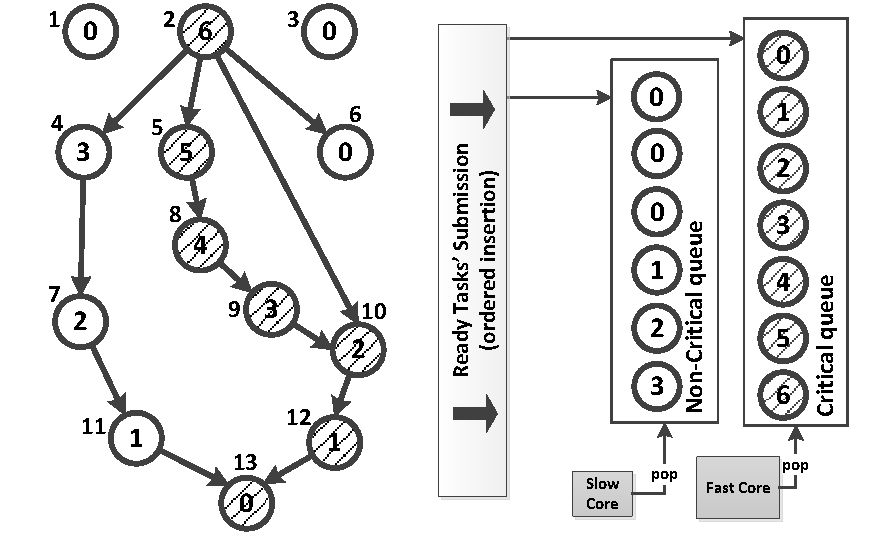
\includegraphics[width=0.6\columnwidth]{Figs/fig_1.pdf} 
\centering
\caption{Task submission with CATS. Nodes are marked with the \textit{bottom level} of each task. Pattern-filled nodes mark the critical tasks.}
\label{botlevels}
\end{figure}


\subsection{Critical Path Scheduler}
\label{sec:cpath}
The Critical Path scheduler (CPATH) dynamically detects the critical path of the TDG.
Like CATS, CPATH separates tasks into two groups: critical and non-critical tasks.
The detected critical tasks are executed by the fast cores in the system and non-critical tasks are executed by slow cores.
The difference with CATS is the algorithm for critical path detection.
CPATH takes into account the task execution time, about which CATS is unaware.
To do so, CPATH implements a more complex and accurate critical path detection algorithm that takes into account task execution time.

CPATH scheduler consists of three steps:
\begin{itemize}

\item \textit{Task prioritization}: this step takes place when a task is finishing its execution (task completion). This is different than CATS since at the end of a task execution the algorithm may record the task execution time (task cost).
%might track a new (unknown) task cost. 
According to the discovered task cost CPATH assigns priorities to tasks by traversing the TDG from top to bottom.

 \item{\textit{Task submission}: when a task becomes \textit{ready}, it is submitted to a \textit{ready queue}. At this point, CPATH decides whether or not the task is \textit{critical} and inserts it in the corresponding ready queue. This step has only slight implementation differences with CATS.}

 \item{\textit{Task-to-core assignment}: this step is identical to CATS and supports the same work stealing mechanisms.}
\end{itemize}
\begin{figure}[tr]
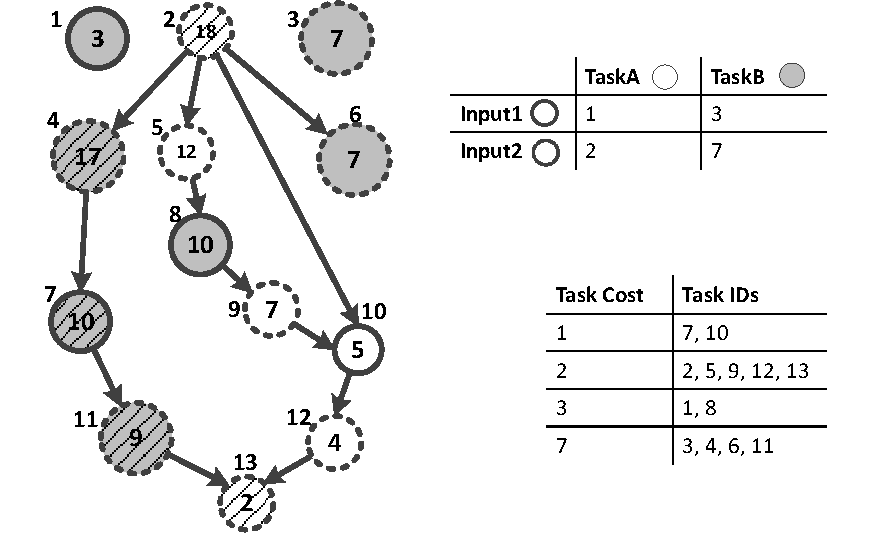
\includegraphics[width=0.6\columnwidth]{Figs/cpath_priorities.pdf} 
\centering
\caption{Priority assignment taking into account the task costs. Task costs are assumed known and are shown in the tables.}
\label{cpath}
\vspace{-0.5cm}
\end{figure}
Figure~\ref{cpath} is used to describe the priority assignment with CPATH.
The specific TDG contains tasks of two different types and two different input sizes.
Node color shows the different task types and the outline of the circle (dashed or solid) shows the different input sizes.
The upper table in Figure~\ref{cpath} indicates the execution time of the tasks according to their type and input size.
The algorithm assumes that task instances of the same type with the same input size have the same (or very similar) execution time.
To track this information, CPATH discovers the cost of every possible task type-input size duple (tt-is duple) that appears on the TDG.
The numbers inside the nodes show the bottom cost-based priorities that CPATH assigns. We define the \textit{bottom cost} of a node on a directed acyclic graph as the maximum estimated time in the dependency chains from this node to a leaf node.The numbers outside the nodes show their task ID.


\subsection{Hybrid Criticality Scheduler}
\label{sec:hybrid}
The Hybrid Criticality Scheduler (HYBRID) is a combination of the CATS and CPATH scheduling policies.
HYBRID keeps the simplicity of the implementation of CATS and introduces the task execution time only if available.
This results in an efficient low-overhead scheduler that computes the critical path of a TDG more faithfully than CATS and with lower overheads than CPATH.
This section describes HYBRID through its relation to CATS and CPATH described in Sections~\ref{sec:cats} and~\ref{sec:cpath}. 
We focus our description on the task prioritization, since task submission and task-to-core assignment for HYBRID are identical to CPATH.

As shown, CPATH computes priorities on task completion. 
The algorithm for priority computation is an expensive operation and is in the critical path of the execution:
on task completion the core becomes available but the start of the next task is delayed by priority computation.
Also, when multiple cores are completing tasks, there will be contention on accessing the TDG for priority computation.
On the other hand, CATS computes priorities during task creation.
The computation of priorities during task creation is more efficient because, unless there is nested parallelism, one core creates all tasks
and therefore there is no contention on priority computation. The downside is that there is potentially less information available 
on task execution time on task creation, as some task type may have not been executed yet at the time all tasks are created.

When comparing CPATH and HYBRID schedulers their logical operation is similar.
However the difference in their implementation may result in different task priorities potentially leading to different schedules.
For applications with small TDGs, HYBRID may not be able to compute an accurate critical path because task creation does not overlap with a sufficient amount of task exits.
Therefore, task execution information will not be available during priority computation and HYBRID will prioritize based on bottom-level priorities (like CATS).
If the application has a large TDG and task creation overlaps with a sufficient amount of task exits, HYBRID will use bottom-cost priorities.

\section{Runtime thread migration mechanisms}

The asymmetry-aware scheduling policies may increase the runtime overheads.
Especially when the runtime operations are executed by the fast cores of the system, preventing them from executing user tasks, the runtime activity can create a bottleneck at the task execution.
This is the motivation for reserving one core responsible for the execution of the runtime activities.
This way the rest of the cores will be devoted for the uninterrupted task execution.
The following subsections describe our motivation and background of this work as well as the current software modifications.
\subsection{Motivation}
\begin{figure}[t]
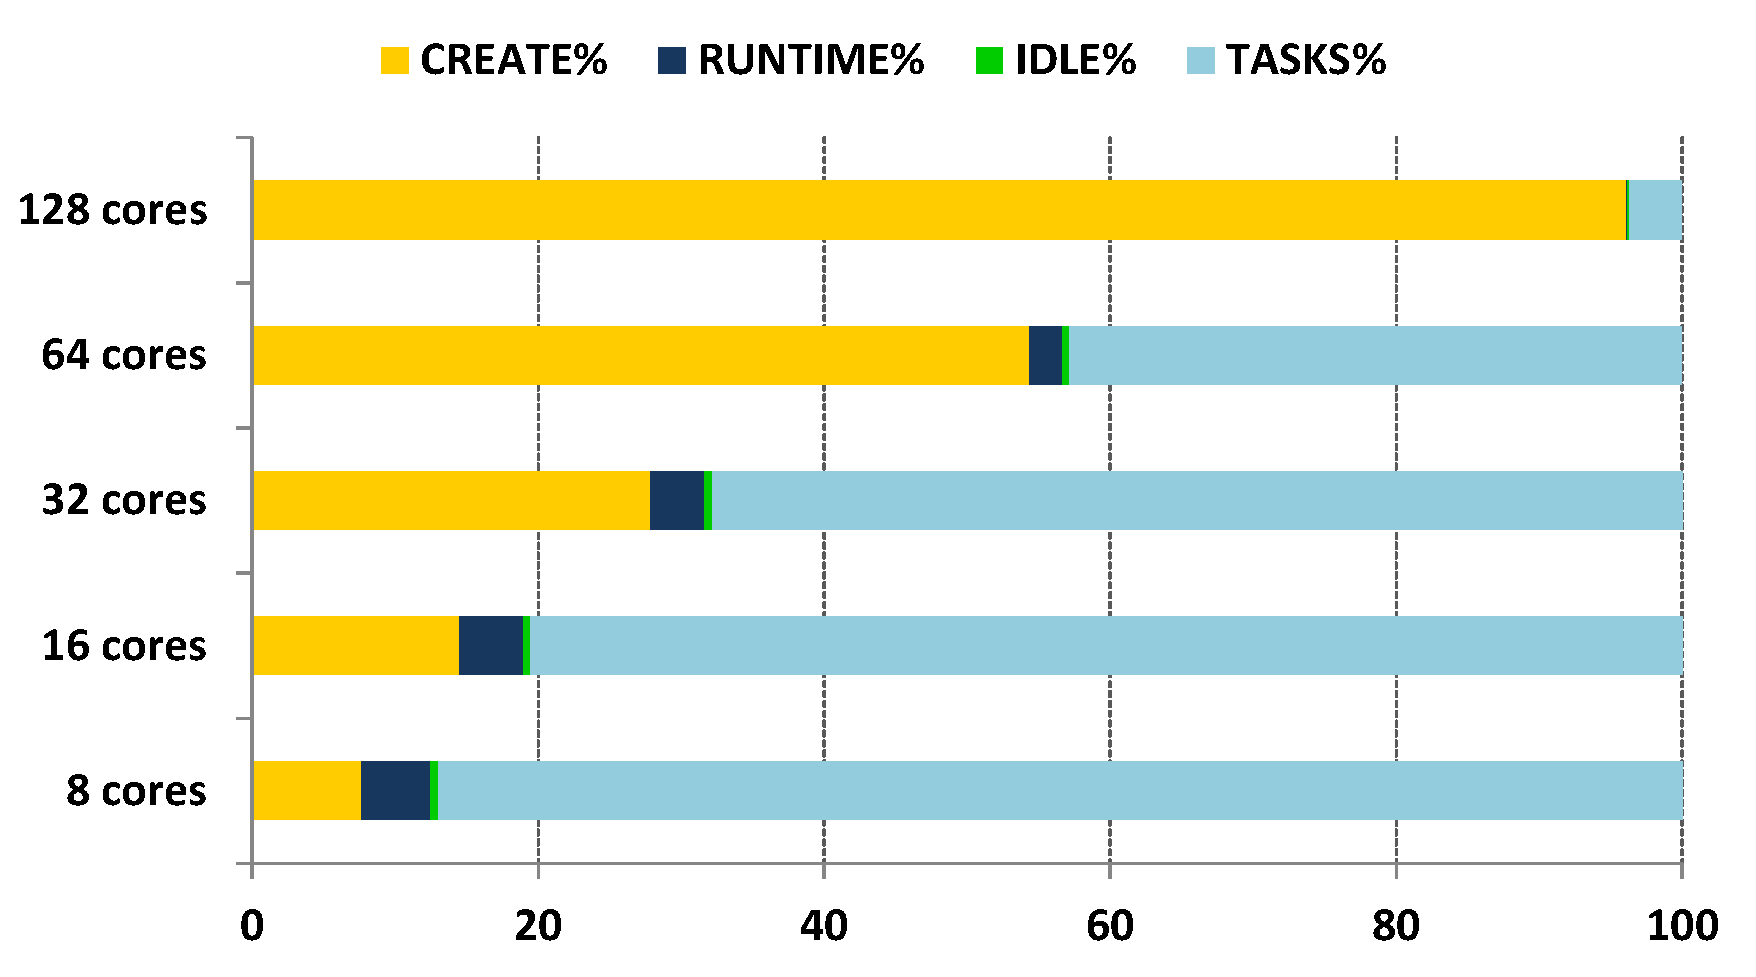
\includegraphics[width=0.6\columnwidth]{Figs/master_thread.pdf} 
\centering
\caption{Activity breakdown of the master thread when executing a parallel application.}
\label{master_activity}
\end{figure}
Task creation is a bottleneck for most applications especially when using smart scheduling policies like the ones we described.
Figure~\ref{fig:master_activity} shows the runtime activity of the master thread during the execution of the Cholesky benchmark on 8, 16, 32, 64 and 128 cores.
Each one of the series represents a different runtime overhead from the ones described above.
CREATE represents the \textit{Creation} step, 
RUNTIME refers to the \textit{Finish} step, IDLE shows the master thread's idle time and the TASKS is the time spent on task execution. 
The percentage of time spent on task creation is increasing as we increase the number of cores.
This is because the creation overhead is static so the more we reduce the application's execution time by adding resources the more important this step becomes in terms of execution time.
On the other hand, the task execution time percentage is decreased as we increase the number of cores because the computational activity is being shared among more resources.
The RUNTIME decreases as we increase the number of cores because this activity is also shared among the resources.

Our motivation for this work is the bottleneck introduced by task creation (CREATION) as shown in Figure~\ref{fig:master_thread}.
We implement a runtime proposal that decouples this piece of the runtime and accelerates it on a specialized hardware resulting in higher performance.

\subsection{Background}

Once again, OmpSs programming model offers the most appropriate environment for exploring this heuristic.
Like OmpSs, task-based parallel programming models\cite{OpenMP4.0:Manual2013},\cite{OmpSs_PPL11}, \cite{OmpSs},  are widely used to facilitate the programming of parallel codes for multi-core systems.
These programming models offer annotations that the programmer can add to the application's sequential code. 
By adding these annotations, the programmer decomposes the application into \textit{tasks} and specifies the input and output data dependencies between them. 
A compiler is responsible to translate the annotations into code by adding calls to the programming model's runtime system. 
The runtime system consists of software threads and is responsible for the efficient execution of the tasks with respect to the data dependencies as well as the availability of resources.
\begin{lstlisting}[float, emph={void,if,return,non_critical_queue, critical_queue,not,true,and,break}, captionpos=b, caption={Compiler generated pseudo-code equivalence for task annotation.},label=task_clause, emph={[2]mat}, emphstyle={[2]}, aboveskip={0\baselineskip}, frame=tb, belowskip={0\baselineskip}]
     ...
  //task_clause
  memalloc(&task, args, size);
  createTask(deps, task, parent, taskData);
     ...
\end{lstlisting}

When the compiler encounters one task annotation in the code, it transforms it to the pseudo-code shown in Listing~\ref{task_clause}.
\texttt{Memalloc} is performing the memory allocation for the task and its arguments.
Next is a runtime call, which is the createTask, responsible for the linking of the task with the runtime system.
At this point a task is considered \textit{created} and below are the three possible states of a task inside the runtime system:
\begin{itemize}
\item \textit{Created:} A task is initialized with the appropriate data and function pointers and it is inserted in the Task Dependency Graph (TDG). The insertion of a task in the TDG implies that the data dependencies of the tasks have been identified and the appropriate data structures have been created and properly initialized. 
\item \textit{Ready:} When all the data dependencies of a created task have been satisfied, the task is ready and it is inserted in the \textit{ready queue} where it waits for execution. 
\item \textit{Finished:} When a task has finished execution and has not been deleted yet.
\end{itemize}

The runtime system creates and manages the software threads for the execution of the tasks. 
Typically one software thread is being bound to each core. 
One of the threads is the \textit{master thread}, and the rest are the \textit{worker threads}. 
The master thread starts executing the code of Listing~\ref{task_clause} sequentially. 
The allocation of the task takes place first.
What follows is the task creation, that includes the analysis of the dependencies of the created task and the connection to the rest of the existing dependencies.
Then, if there are no task dependencies, which means that the task is ready, the task is also inserted in the ready queue and waits for execution.

Listing~\ref{taskCreation} shows the pseudo-code for the task creation step within the runtime.
The \texttt{createTask} function is first initializing the task by copying the corresponding data to the allocated memory as well as connecting the task to its parent task (\texttt{initAndSetupTask}).
After this step, the task is ready to be inserted in the TDG; this is done by the \texttt{insertToTDG} function.
This function takes as arguments a list with all the memory addresses that are to be written or read by the task (\texttt{dList}), and the task itself.
If for a task the \texttt{dList} is empty, this means that there are no memory addresses that need to be tracked during the execution; thus, the task is marked as \textit{ready} by inserting it in the \textit{ready queue} (\texttt{rQueue\_submission}).
Each entry of \texttt{dList} contains the actual memory address as well as the access type (read, write or read-write).
The runtime keeps a unified dependency tracking structure (\texttt{depMap}) where it stores all the tracked memory addresses together with their writer and reader tasks.
For each item in the \texttt{dList} the runtime searches for an existing representation inside the \texttt{depMap}.
If the memory address of an entry of the \texttt{dList} is not represented in the \texttt{depMap}, it is being added;
if the address of a \texttt{dList} item belongs to the \texttt{depMap}, this means that a prior task has already referred to this memory location. 
Thus at this point there is a data dependency.
Then according to the type of the access type of \texttt{d}, the readers and the writers of the specific address are updated in the \texttt{depMap}.

To reduce the lookup into the \texttt{depMap} calls, every time a memory address is modified, the tasks keep track of their \textit{successors} as well as the number of \textit{predecessors}.
The \textit{successors} of a task are all the tasks that their input depends on the output of the current task.
The \textit{predecessors} of a task are the tasks whose output is used as input for the current task.
When a \texttt{read} access is identified, the task that is being created is added to the list of successors of the last writer task (lineXX).

As tasks are executed, the dependencies between them and their successors are satisfied. 
So the successor tasks that are waiting for input, eventually become \textit{ready} and are inserted to the ready queue.
When a task becomes \textit{finished}, the runtime has to perform some actions in order to prepare the successor tasks for execution.
These actions are described in Listing~\ref{taskFinish}.
The runtime first updates the \texttt{depMap} to remove the possible references of the task as reader or writer.
Then, if the task does not have any successors, it can safely be deleted.
If the task has successors, the runtime traverses the successor list and for each successor task it decreases its predecessor counter.
If for a successor task its predecessor counter reaches zero, then this task becomes \textit{ready} and it is inserted in the ready queue (\texttt{rQueue\_submission(succ)}).

To summarize, the runtime activity mainly takes place at the task state changes. 
One state change corresponds to the task creation, so a task from being just allocated it becomes created, and the second change occurs when a task from being ready becomes finished. 
In these two runtime phases the runtime system interferes and introduces runtime overheads.


\begin{lstlisting}[float, emph={void,if,return,not,true,and,break}, captionpos=b, caption={Pseudo-code for task creation.},label=taskCreation, emph={[2]mat}, emphstyle={[2]}, aboveskip={0\baselineskip}, frame=tb, belowskip={0\baselineskip}]

void createTask(Deplist dList, Task task1, 
            Task parent, Data taskData) {
  initAndSetupTask(task1, parent, taskData);
  insertToTDG(dList, task1);
}

Dependency depMap[];

void insertToTDG(DepList dList, Task task1) {
 if( dList.empty() ) {
   rQueue_submission(task1);
   return;
 }
 Dependency entry;
 for( d in dList ) {
   entry = depMap.lookupAddress(d.address());
   if(entry == NULL) 
     depMap.add(d.address(), d.accessType(), task1);
   if(d.accessType() == "write") {
     entry.addLastWriter(task1);
   }
   else if(d.accessType() == "read") {
     entry.addReader(task1);
     entry.lastWriter()->addSuccessor(task1);
   }
   else if(d.accessType() == "read-write") {
     entry.addLastWriter(task1);
     entry.addReader(task1);
   }

 }
}
\end{lstlisting}

\begin{lstlisting}[float, emph={void,if,return,not,true,and,break}, captionpos=b, caption={Pseudo-code for task$\_$finish runtime activity.},label=taskFinish, emph={[2]mat}, emphstyle={[2]}, aboveskip={0\baselineskip}, frame=tb, belowskip={0\baselineskip}]
void task_finish(Task *t) {
  depMap.deleteAsWriter(t);
  depMap.deleteAsReader(t);
  if(t->successors.empty()) delete task;
  else {
    for( succ in t->successors ) {
      succ.decreasePredecessors();
      if(succ.numPredecessors == 0) 
        rQueue_submission(succ);
    }
  }
\end{lstlisting}

\subsection{Runtime Activity Manager}
RAM assumes the existence of a specialized hardware that accelerates the task creation step.
RAM relieves the master and worker threads from this intensive runtime activity by offloading it on the special purpose hardware.
In our design, apart from the master and the worker threads, we introduce the Special Runtime Thread (SRT). 
When the runtime system starts, it creates the SRT and binds it to the task creation accelerator, keeping its thread id in order to manage the usage of it.
During runtime, the master and worker threads look for ready tasks in the task ready queue and execute them along with the runtime.
SRT, instead of querying the ready queue for tasks, it looks for runtime activity requests in the runtime ready queue (RRQ) and if there are requests, it executes them.

Figure~\ref{fig:communication} shows the communication infrastructure between threads within our runtime.
Our system maintains two queues; the ready task queue (\texttt{TASKQ}) and the runtime requests queue (\texttt{RRQ}).
The TASKQ is used to keep the tasks that are ready for execution. 
The RRQ is used to keep the runtime activity requests. 
The master and the worker threads can push and pop tasks to and from the TASKQ and they can also add runtime activity to the RRQ. 
The special runtime thread (SRT) pops runtime requests from the RRQ and under circumstances, it also pops ready tasks from the TASKQ.

When the master thread encounters a task clause in the application's code, after allocating the memory needed, it calls the \texttt{createTask} as shown in Listing~\ref{createTask} and as described in Section~\ref{sec.background}. 
RAM decouples the execution of \texttt{createTask} from the master thread. To do so, when a thread encounters a call to the \texttt{createTask}, the runtime system checks if the SRT is enabled; if so, instead of performing the task creation itself, it generates a \textit{CREATE} request and inserts it in the RRQ so that the SRT can read and execute it. The running thread then continues by executing tasks. 
The \textit{CREATE} runtime request includes the appropriate info to execute the code described in Listing~\ref{taskCreation}.
That is, the dependence analysis data, the address of the allocated task, its parent and the taskData.

\begin{lstlisting}[float, emph={void,if,return,non_critical_queue, critical_queue,not,true,and,break}, captionpos=b, caption={Pseudo-code for the SRT loop.},label=SRTloop, emph={[2]mat}, emphstyle={[2]}, aboveskip={0\baselineskip}, frame=tb, belowskip={0\baselineskip}]
1 void SRTloop() {
   int maxTasks = runtime.numWorkers * MAX;
2  while( true ) {   
3    while( not RRQ.empty() ) {
4      executeRequest( RRQ.pop() );
5    if( RRQ.empty() and readyTasks > maxTasks )
7      executeTask( readyQ.pop() );
8  }
9  if( runtime.SRTstop() ) break;
10 return; 
11}  
\end{lstlisting}

\begin{figure}[t]%
	\centering
	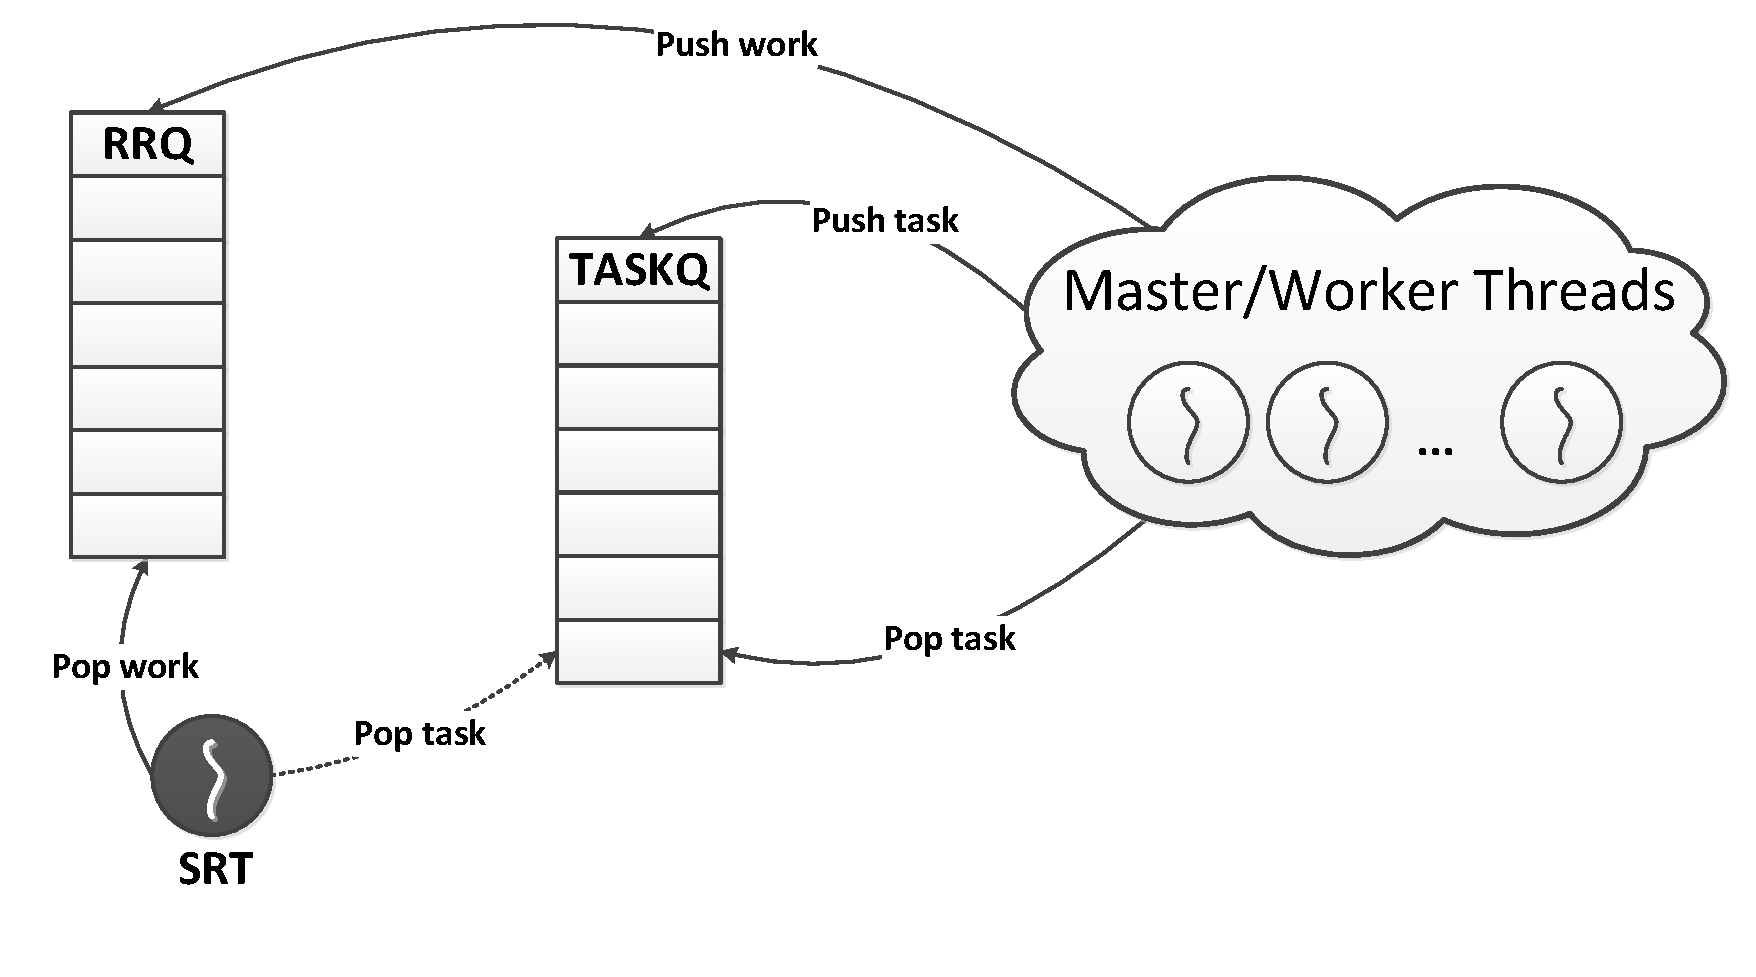
\includegraphics[width=1.0\columnwidth]{Figs/communication.pdf}
	\vspace{-0.5cm}
	\caption{Communication mechanism between master/workers and SRT threads.}
	\label{fig:communication}%
	\vspace{-0.3cm}
\end{figure}
At the same time that the master and worker threads are executing tasks, the SRT is looking for \textit{CREATE} requests in the RRQ to execute.
Listing~\ref{SRTloop} shows the code that the SRT is executing until the end of the parallel execution.
The special runtime thread continuously checks whether there are requests in the RRQ (line 3). As long as there is a pending task creation, the SRT executes the task submission and inserts the task in the TDG with a call to the \texttt{executeRequest} (line 4). If at some point the RRQ becomes empty, the SRT checks the number of ready tasks in the ready queue (lines 5, 6) and if the number of ready tasks is greater than \texttt{maxTasks}, which means that the workers are very loaded, it executes the next ready tasks in the queue. 




\section{Asymmetry-aware runtime system}

Having completed the previous steps we plan to combine our implementations of scheduling techniques and runtime thread migration mechanisms and end up with a novel runtime system for asymmetric architectures that offers two levels of adaptability: first is the choice of the appropriate core type for the runtime execution and second is the appropriate scheduling of the tasks on the available cores.

The first step in discovering the appropriate scheduling-migration mechanism combination is to perform experiments of scientific applications using all the possible combinations of migration and scheduling policies as well as use different machine set-ups in terms of numbers of fast and slow cores.
The analysis of these results will show us whether the combining existing implementations is efficient and under what circumstances.
After concluding to the most appropriate mechanism, we will further verify the results on a larger scale, using an HPC machine with a larger number of cores.


\section{Thesis Roadmap}
The Gantt graph below describes the whole plan with the various stages. 
Each stage corresponds to a section of this chapter. 
The literature review process (named Related works in the graph) is a constant activity that lasts the entire course of the PhD.

A part of work for this PhD was conducted before the PhD enrolment.
This work is described in the graph thus the graph starts from September of 2014.
However, as is noted on the graph, the official PhD enrolment is on September of 2015.

The Gantt graph below has been updated with the current status of the publications. 
During this year, we successfully published the Journal of Scheduling policies.
Furthermore we modified improved and submitted the paper "Asymmetric System Analysis" to multiple conferences but none of them has accepted our work so far.
We plan to perform further modifications in the text and resubmit the paper this October.
In addition, we are in progress of writing the paper for the Runtime Thread Migration and submit it in October as well.


~\\ \\ \\
\noindent\resizebox{\textwidth}{!}{
\begin{ganttchart}[vgrid,hgrid, 
today=37,
today offset=.32,
today label=Current Month,
today rule/.style=%
{draw=blue, ultra thick},
milestone label font=\Large,
group label font=\Large,
title label font=\Large,
bar label font=\Large, 
bar/.append style={fill=green!90}]{1}{52}
%\begin{ganttchart}[vgrid,hgrid, group right shift=0, group top shift=0.7, group height=.3, group peaks width={0.2}]{1}{40}
    \gantttitle{2014}{4}
	\gantttitle{2015}{12} 
	\gantttitle{2016}{12} 
	\gantttitle{2017}{12} 
	\gantttitle{2018}{12} \\
	\gantttitlelist{9,...,12}{1} 
	\gantttitlelist{1,...,12}{1}
	\gantttitlelist{1,...,12}{1}
	\gantttitlelist{1,...,12}{1}
	\gantttitlelist{1,...,12}{1} \\
	\ganttbar{Related works}{1}{52}\\
%	\ganttmilestone{PhD enrolment}{12}\\
	\ganttgroup{\textbf{Scheduling Policies}}{1}{19}\\ %1
	\ganttbar{CATS Scheduler}{1}{9} \\ %2
	\ganttmilestone{\textit{CATS paper}}{9}\\ %3
	\ganttlink{elem2}{elem3}
	\ganttbar{Journal for Scheduling Policies}{9}{19}\\ %4
	\ganttmilestone{\textit{Scheduling policies journal}}{31}\\ %5
	\ganttlink{elem4}{elem5}
	\ganttgroup{\textbf{Asymmetric system analysis}}{13}{24}\\ %6
	\ganttbar{Evaluation and Exploration}{13}{18}\\ %7
	\ganttlinkedbar{Paper writing and submission}{19}{24}\\ %8
	\ganttlinkedbar{Paper review and modification}{24}{38}\\%9
	\ganttmilestone{\textit{Exploration paper}}{45}\\ %10
	\ganttlink{elem9}{elem10}
	\ganttgroup{\textbf{Runtime Thread Migration (RTM)}}{21}{31}\\ %10
	\ganttbar{Implementation and Optimization}{21}{25}\\ %11
	\ganttbar{Evaluation}{26}{27}\\ %12
	\ganttbar{Paper writing for RTM}{27}{38}\\ %13
	\ganttmilestone{\textit{Paper for RTM}}{44}\\ %14
	\ganttlink{elem14}{elem15}
	\ganttgroup{\textbf{Asymmetry Aware Runtime (AAR)}}{31}{44}\\ %15
	\ganttbar{Porting schedulers in runtime}{31}{33}\\ %16
	\ganttbar{Experiments and Optimization}{34}{39}\\ %17	
	\ganttbar{Final evaluation of AAR}{40}{42}\\ %18
	\ganttbar{Paper writing for AAR}{42}{44}\\ %19
	\ganttmilestone{\textit{Paper for AAR}}{52}\\ %20
    \ganttlink{elem20}{elem21}	
	\ganttbar{Thesis writing and defense}{45}{52}		
\end{ganttchart}

\if 0
\begin{ganttchart}[vgrid,hgrid,bar/.append style={fill=green!90}]{1}{52}
%\begin{ganttchart}[vgrid,hgrid, group right shift=0, group top shift=0.7, group height=.3, group peaks width={0.2}]{1}{40}
    \gantttitle{2014}{4}
	\gantttitle{2015}{12} 
	\gantttitle{2016}{12} 
	\gantttitle{2017}{12} 
	\gantttitle{2018}{12} \\
	\gantttitlelist{9,...,12}{1} 
	\gantttitlelist{1,...,12}{1}
	\gantttitlelist{1,...,12}{1}
	\gantttitlelist{1,...,12}{1}
	\gantttitlelist{1,...,12}{1} \\
	\ganttbar{Related works}{1}{52}\\
	\ganttmilestone{PhD enrolment}{12}\\
	\ganttgroup{\textbf{Scheduling Policies}}{1}{19}\\ %1
	\ganttbar{CATS Scheduler}{1}{9} \\ %2
	\ganttmilestone{\textit{CATS paper}}{9}\\ %3
	\ganttlink{elem2}{elem3}
	\ganttbar{Journal for Scheduling Policies}{9}{19}\\ %4
	\ganttmilestone{\textit{Scheduling policies journal}}{31}\\ %5
	\ganttlink{elem4}{elem5}
	\ganttgroup{\textbf{Asymmetric system analysis}}{13}{24}\\ %6
	\ganttbar{Evaluation and Exploration}{13}{18}\\ %7
	\ganttlinkedbar{Paper writing and submission}{19}{24}\\ %8
	\ganttmilestone{\textit{Exploration paper}}{26}\\ %9
	\ganttlink{elem8}{elem9}
	\ganttgroup{\textbf{Runtime Thread Migration (RTM)}}{21}{31}\\ %10
	\ganttbar{Implementation and Optimization}{21}{25}\\ %11
	\ganttbar{Evaluation}{26}{27}\\ %12
	\ganttbar{Paper writing for RTM}{27}{31}\\ %13
	\ganttmilestone{\textit{Paper for RTM}}{39}\\ %14
	\ganttlink{elem13}{elem14}
	\ganttgroup{\textbf{Asymmetry Aware Runtime (AAR)}}{31}{44}\\ %15
	\ganttbar{Porting schedulers in runtime}{31}{33}\\ %16
	\ganttbar{Experiments and Optimization}{34}{39}\\ %17	
	\ganttbar{Final evaluation of AAR}{40}{42}\\ %18
	\ganttbar{Paper writing for AAR}{42}{44}\\ %19
	\ganttmilestone{\textit{Paper for AAR}}{52}\\ %20
    \ganttlink{elem19}{elem20}	
	\ganttbar{Thesis writing and defense}{45}{52}	
	
\end{ganttchart}
\fi
}


\chapter{Methodology}

% **************************** Define Graphics Path **************************
\ifpdf
	\graphicspath{{Chapter5/Figs/Raster/}{Chapter5/Figs/PDF/}{Chapter5/Figs/guided/}{Chapter5/Figs/unguided/}}
\else
    \graphicspath{{Chapter5/Figs/Vector/}{Chapter5/Figs/}}
\fi

\section{The OmpSs programming model}
\label{sec:ompss}
We choose to implement the new mechanisms proposed in this document in the OmpSs programming model.
The OmpSs programming model is a task-based programming model that offers a high level abstraction to the implementation of parallel applications for various homogeneous and heterogeneous architectures~\cite{OmpSs_PPL11,OmpSs}. It enables the annotation of code blocks or function declarations with the task directive, which declares a task. Every invocation of such a function creates a task that is executed concurrently with other tasks or parallel loops. OmpSs also supports task dependencies and dependency tracking mechanisms~\cite{StarSs}. 
OmpSs is composed of two main elements: the Mercurium compiler, responsible for the translation of the OmpSs annotation clauses to source code that calls to the Nanos++ API, and the Nanos++ runtime system, responsible for the internal creation and execution of the tasks. 
%OmpSs is built with the support of the Mercurium compiler, responsible for the translation of the OmpSs annotation clauses to source code, and the Nanos++ runtime system, responsible for the internal creation and execution of the tasks.

Nanos++ is an environment that serves as the runtime platform of OmpSs. It provides device support for heterogeneity and includes different plug-ins for implementations of schedulers, throttling policies, barriers, dependency tracking mechanisms, work-sharing and instrumentation. This design allows to maintain the runtime features by adding or removing plug-ins, facilitating the implementation of a new scheduler, or the support of a new architecture.

The implementations of the different scheduling policies in Nanos++ perform various actions on the states of the tasks. A task is \textit{created} if a call to this task is invoked but it is waiting until all its inputs are produced by previous tasks. When all the input dependencies are satisfied, the task becomes \textit{ready}. The ready tasks of the application at a given point in time are inserted in the \textit{ready queues} as stated by the scheduling policy. Ready queues can be thread-private or shared among threads. When a thread becomes idle, the scheduling policy picks a task from the ready queues for that thread to execute. The default OmpSs scheduler employs a \textit{breadth-first} policy~(BF)~\cite{Duran_schedulers_08} and implements a single first-in-first-out ready queue shared among all threads. When a task is ready, it is inserted in the tail of the ready queue and when a core becomes available, it retrieves a task from the head of the queue. BF does not differentiate among core types and assigns tasks in a first-come-first-served basis. We use this scheduler as our baseline.

The Nanos++ internal data structures support task prioritization. The task priority is an integer field inside the task descriptor that rates the importance of the task. If the scheduling policy supports priorities, the ready queues are implemented as \textit{priority queues}. In a priority queue, tasks are sorted in a decreasing order of their priority. The insertion in a priority queue is always ordered and the removal of a task is always from the head of the queue, i.e., the task with the highest priority. The priority of a task can be either set in user code, by using the \textit{priority} clause, which accepts an integer priority value or expression, or dynamically  by the scheduling policy, as is described in the next section.

Nanos++ runtime is the baseline of our runtime implementations.
We choose to implement our proposed scheduling policies within this runtime.
Also Nanos++ is easy to modify in order to reserve one thread responsible for the runtime.





\section{Evaluation}
\subsection{Evaluation platform}
\label{sec:platform}
The Hardkernel ODROID-XU3 development board has an 8-core Samsung Exynos 5422 chip with an ARM big.LITTLE architecture and 2GB of LPDDR3 RAM at 933MHz. The chip has four Cortex-A15 cores at 2.0GHz and four Cortex-A7 cores at 1.4GHz. The four Cortex-A15 cores form a \textit{cluster} with a shared 2MB L2 cache, and the Cortex-A7 share a 512KB L2 cache. The two \textit{clusters} are coherent, so a single shared memory application can run on both clusters, using up to eight cores simultaneously. In our experiments, we evaluate a set of possible combinations of fast and slow cores varying the total number of cores from two to eight. For the reminder of the paper, we refer to Cortex-A15 cores as \textit{big} and to Cortex-A7 cores as \textit{little}.

\subsection{Simulator}

To evaluate our approaches on larger multi-core systems we use the heterogeneous multi-core TaskSim simulator~\cite{AbstrLevels_TACO12}. 
TaskSim allows the specification of a heterogeneous system with two different types of cores: fast and slow. 
We can configure the amount of cores of each type and the difference in performance between the different types (performance ratio) in the TaskSim configuration file.
In our experiments, we will use up to a total of 80 distinct heterogeneous machine configurations.  
These comprise systems with the total number of cores ranging from 16 to 128, and the number of fast cores ranging from 1 to 16. 
For all these configurations, we evaluate the following performance ratios between fast and slow cores: 2$\times$, 2.5$\times$, 3$\times$, 3.5$\times$ and 4$\times$.

\subsection{Applications}
\label{sec:applications}
\begin{table*}[!t]
	\centering
	\scriptsize
	\caption{Evaluated benchmarks from the PARSEC benchmark suite}
	
	\setlength{\tabcolsep}{4pt}
	\begin{tabular}{|p{1.3cm}|p{7cm}|p{3cm}|p{1.6cm}|p{1cm}|}
	\hline
	\textbf{Benchmark} & \multicolumn{1}{|c|}{\textbf{Description}} & \multicolumn{1}{|c|}{\textbf{Input}} & \textbf{Parallelization} &\multicolumn{1}{|c|}{\textbf{Perf ratio}} \\
	\hline \hline
	blackscholes & Calculates the prices for a portfolio of European options analytically with the Black-Scholes partial differential equation. & 10,000,000 options & data-parallel &2.18 \\ \hline
	bodytrack & Computer vision application which tracks a 3D pose of a marker-less human body with multiple cameras through an image sequence. & 4 cameras, 261 frames, 4,000 particles, 5 annealing layers & pipeline & 4.16 \\ \hline
	canneal & Simulated cache-aware annealing to optimize routing cost of a chip design. & 2.5 million elements, 6,000 temperature steps & unstructured & 1.73 \\ \hline
	dedup & Compresses a data stream with a combination of global compression and local compression in order to achieve high compression ratios. & 351 MB data & pipeline & 2.67 \\ \hline
	facesim & Takes a model of a human face and a time sequence of muscle activation and computes a visually realistic animation of the modeled face. & 100 frames, 372,126 tetrahedra & data-parallel & 3.40 \\ \hline
	ferret & Content-based similarity search of feature-rich data (audio, images, video, 3D shapes, etc.) & 3,500 queries, 59,695 images database, find top 50 images & pipeline & 3.59 \\ \hline
	fluidanimate & Uses an extension of the Smoothed Particle Hydrodynamics method to simulate an incompressible fluid for interactive animation purposes. & 500 frames, 500,000 particles & data-parallel & 2.64 \\ \hline
	streamcluster & Solves the online clustering problem. & 200,000 points per block, 5 block & data-parallel & 3.48 \\ \hline
	swaptions & Intel RMS workload which uses the Heath-Jarrow-Morton (HJM) framework to price a portfolio of swaptions. & 128 swaptions, 1 million  simulations & data-parallel & 2.78 \\ \hline
	\end{tabular}
	\label{tab:parsec}
	\vspace{-0.3cm}
\end{table*}

In our experiments we use the PARSECSs benchmark suite~\cite{Chasapis:TACO2016}.
This benchmark suite offers a set of scientific real world applications implemented in OmpSs as well as pthreads. 
Table~\ref{tab:parsec} shows the applications and their characteristics.

Apart from the PARSECSs benchmark suite we use four scientific kernels implemented in the OmpSs programming model: Cholesky factorization, QR factorization, Heat diffusion and Integral Histogram. These benchmarks are accessible in the BSC Application Repository~\cite{BAR}. 

\textbf{Cholesky factorization} is a dense matrix operation that is used for solving linear equations in linear least square systems.
The OmpSs implementation of Cholesky blocks the input matrix into square blocks of floats and each task is responsible for performing the factorization on one block.

\textbf{QR Factorization} is a linear algebra algorithm that is used to solve the linear least squares problem \cite{QR}. 
We evaluate the performance of a blocked, communication avoiding QR implementation in OmpSs. 
We use an input blocked matrix of 8192$\times$8192 doubles forming 16$\times$16 blocks.

%\subsubsection{Heat Diffusion}
\textbf{Heat diffusion} uses the Gauss-Seidel method to compute the heat distribution on a matrix from \textit{x} heat sources. Heat diffusion implements an iterative solver of the equation that invokes the Gauss-Seidel method until the desired convergence is reached. We use a matrix of 8192$\times$8192 doubles and block size of 512$\times$512.

\textbf{Integral histogram} is a method to compute a cumulative histogram for each pixel of an image. 
The OmpSs implementation performs 
a horizontal and a vertical scan that transmit histograms to the blocks that reside on the right or below the current block.
Due to these transmissions, the application introduces many task dependencies. We use as input an image of 4096$\times$4096 pixels and block size of 512$\times$512.

\textbf{Blackscholes} from the PARSEC Benchmark Suite~\cite{Bienia:PhD2011}, is an Intel RMS benchmark. It calculates the prices for a portfolio of European options analytically with the Black-Scholes partial differential equation (PDE).
The OmpSs implementation~\cite{AbstrLevels_TACO12}, divides the work into units of a predefined block size. 
This block size allows having much more task instances than threads, which implies a much better load balance, as this is an embarrassingly parallel application with no dependencies among tasks in the same run.


\subsection{Metrics}
\label{sec:metrics}

All the experiments in this paper are performed on the Hardkernel Odroid XU3 described in Section~\ref{sec:platform}. In our experiments, we make use of the \texttt{cpufreq} driver to set the big cores to run at 1.6GHz and the little cores at 800MHz. 

\subsubsection{Performance}
To estimate the impact of the different kinds of cores, we evaluate seven configurations with different numbers of \textit{little} (L) and \textit{big} (B) cores, denoted \texttt{L+B}.
For each configuration and benchmark, we report the average performance of five executions taking into account only the parallel region of the application. Then, we report the speedup of the application over its serial execution time on one little core.
Equation~\ref{eq.speedup} shows the formula to compute the speedup.
\begingroup\makeatletter\def\f@size{9}\check@mathfonts
\begin{equation}
  \text{Speedup(L, B, method)} = \frac{\text{Exec. time(1, 0, serial)}}{\text{Exec. time(L, B, method)}}
\label{eq.speedup}
\end{equation}
\endgroup

\subsubsection{Power and Energy}
In this platform, there are four separated current sensors to measure in real time the power consumption of the cluster of A15 cores, the cluster of A7 cores, the GPU and DRAM. 
To gather the power and energy measurements, a background daemon is reading the machine power sensors periodically during the application execution with negligible overhead. Sensors are read every 0.27 seconds, and their values are written in a file. With the help of timestamps, we correlate the power measurements with the parallel region of the application in a  \emph{post-mortem} process. The reported power consumption is the average power that the SoC was consuming during five executions of each configuration, considering only the parallel region of the application. We then report the average power in Watts during the execution. 

Finally, in terms of energy and EDP, we report the total energy and EDP of the benchmark's region of interest normalized to the value that it consumes when running on four little cores with static threading.
Equations~\ref{eq.energy} and~\ref{eq.edp} show the formulas for these calculations.
\begingroup\makeatletter\def\f@size{8}\check@mathfonts
\begin{equation}
  \text{Normalized Energy(L, B, method)} = \frac{\text{Energy(L, B, method)}}{\text{Energy(4, 0, static-threading)}}
  \label{eq.energy}
\end{equation}
\begin{equation}
  \text{Normalized EDP(L, B, method)} = \frac{\text{EDP(L, B, method)}}{\text{EDP(4, 0, static-threading)}}
  \label{eq.edp}
\end{equation}
\endgroup

\subsection{Results}
\label{sec:results}

We have already made some progress in this thesis and have already covered some of the work to be done.
From our evaluation of the asymmetric system described in Section~\ref{sec:asymmetric} we found that adding little cores to a symmetric multi-core with big cores presents significant challenges for the application, OS and runtime developers. Little cores increase load imbalance and can degrade performance as a result. Relying on the application developer to deal with this asymmetry is complex and many applications are not ready. A dynamic OS scheduler such as \emph{GTS} can help in mitigating these problems, but the best results in terms of performance are obtained with the \emph{Task-based} approach. In terms of power and energy, the asymmetric multi-core provides significant benefits, although the symmetric multi-core with little cores remains the most energy-efficient configuration. The \emph{Task based} approach offers the highest performance with the lowest energy consumption when used on our 8-core system. With this in mind, the system-aware scheduling policies of a task-based programming model are meant to improve scheduling at the most appropriate level of the software stack.




\subsubsection{Evaluation of Scheduling Policies}
This section shows the results obtained from our scheduling policies described in Section~\ref{sec:scheduling}.
We compare our approaches against a dynamic implementation of the Heterogeneous Earliest Finish Time scheduler~\cite{HEFT} (dHEFT) in the OmpSs programming model.
The implementation assumes two different types of cores (big and
little) and keeps records of the tasks’ execution times in each core. The original HEFT~\cite{HEFT} implementation assumes the
prior knowledge of the TDG as well as the costs of the tasks.
In our case, since the evaluation consists of running real applications, the best way to compare HEFT to our proposal is
to keep the scheduling idea of HEFT and transform it from
a static to a dynamic scheduler. This means that dHEFT
discovers the costs of the tasks at runtime, computes a mean
value of the costs for each task-type and parameter-size duple for each type of core, and then finds the core that will
finish the task at the earliest possible time. 

To find the earliest possible executor, dHEFT maintains
one list per core (wlist) including the ready tasks waiting
to be executed by that core. When another task becomes
ready, dHEFT first checks if there are records of prior execution of this task. If the number of records is sufficient
(in our experiments we require a minimum of three records)
then the estimated execution time of the task is considered
stable. Then, using that estimated execution time, the task
is scheduled to the earliest executor by consulting the wlist
of all the cores. If the number of records is not sufficient
for one of the core types, then the task is scheduled to the
earliest executor of this core type to get another record of
that task-type and core-type execution time. In all cases,
dHEFT updates the history of records on every task execution to adapt for phase changes in the application.

We evaluate the applications Cholesky, QR, Heat diffusion, Integral Histogram and Bodytrack described in Section~\ref{sec:applications}.
To more precisely characterise the benchmarks, we plot the task cost variability for each benchmark on Figure~\ref{distributions}.
For each of these plots, the $x$ axis shows the normalized task cost and the $y$ axis the number of tasks that correspond to this task cost (e.g. how many tasks have this cost).
This is used to show how heterogeneous each application is and explain the behaviour of the heterogeneous schedulers that take into account the execution time.

Figure~\ref{speedup} shows the speedup obtained for each application,  scheduler and machine set-up.
The x axis shows for each application the total number of cores at the bottom and the number of big cores at the top.
We classify the benchmarks according to their task cost variability to easier explain the results.

%------ HEAT ---------- very low variability


Heat diffusion is the kernel with the lowest task variability (e.g. the most homogeneous benchmark) as shown in Figure~\ref{heat_dist}.
CATS, HYBRID and dHEFT increase the performance of heat by 10\% on 8 cores and obtain similar results for the other numbers of cores by rearranging the tasks according to the type of the resources.
Due to its high per-task overheads and the homogeneity of the benchmark, CPATH scheduler cannot outperform the random BF scheduler. 
Moreover, for this benchmark, CPATH detects only 23\% of the tasks to be critical while CATS and HYBRID detect approximately 54\%, when running on 8 cores.
This happens because with CPATH, it is more likely to have zero-priority tasks during the task submission step, due to the post-exit task priority assignment that the algorithm introduces. 
The zero-priority tasks are considered non-critical and this limits the utilization of the big cores with CPATH. 

%---------- CHOLESKY 16x16 ------------ low variability

Cholesky 16$\times$16 has also low task cost variability. 
The improvements of CATS, dHEFT and HYBRID over BF are limited to around 7\% when running on 8 cores.
These schedulers perform almost the same for the rest numbers of cores and CPATH performs almost the same as BF. 
The increased overheads of CPATH do not pay off with better schedules since, for the same reason as in the case of Heat diffusion, only 10\% of the tasks are marked as critical on 8 cores (while 21\% CATS and 16\% HYBRID).

%--------- BODYTRACK --------------- low variability - very high number of tasks

Bodytrack shows low task cost variability, since 99\% of its tasks have similar execution times.
In this case, contrarily to the previous benchmarks CPATH manages to achieve similar speedups to CATS and HYBRID and outperform BF by up to 15\%.
This is due to the very high number of tasks of bodytrack; CPATH overcomes its overheads by using the detected task execution times for a higher number of tasks.
In other words, the learning phase of CPATH becomes a smaller proportion of the total execution of the benchmark.
Since bodytrack has so many tasks, the per-task overhead of CPATH is around 120us while for CATS it is 93us.
On the other hand, dHEFT shows poor performance because of the overheads of analyzing a TDG with a high number of tasks to compute the earliest finish time schedule.

%---------- HISTOGRAM --------------- medium variability - good amount of tasks (2048)

Integral histogram is characterized by medium task cost variability and high amount of tasks.
This benchmark is dependency intensive with limited parallelism, which makes scheduling decisions very important.
CATS and HYBRID schedulers achieve the best results since they focus more on the TDG structure and dependencies, improving BF by 30\% and 27\% respectively.
CPATH and dHEFT are slightly less efficient and improve BF by 19 and 21\% respectively.

%---------- CHOLESKY 8x8 -------------- high variability but very few tasks

For Cholesky 8$\times$8, the heterogeneous schedulers CATS, HYBRID and dHEFT constantly improve the performance of BF and reach up to 45\% improvement on 8 cores.
It is observed here that dHEFT indeed performs better when the number of tasks is limited as this workload has 120 tasks in total.
The additional overheads of CPATH do not compensate with increased performance in this case because there are not enough tasks to apply the better scheduling.

%---------------- QR ------------ the highest variability and good number of tasks (1496)

QR factorization is the highest task cost variability benchmark as shown in Figure~\ref{qr_dist}.
This is the reason why HYBRID gradually outperforms CATS as we increase the number of cores.
%With a small additional overhead,
%(CATS: 1419us while HYBRID: 14514us per-task overhead)
%as Table~\ref{tab.apps} shows, 
HYBRID manages to efficiently detect critical tasks that reside on the critical path and boost their execution reaching 17\% improvement over the baseline.
For this benchmark, CPATH also reaches a 13\% improvement over BF since task cost matters in this case. 
However, CPATH speedup is still limited compared to HYBRID because of the higher scheduling overheads which in this case is 1.8$\times$ higher than CATS overheads.
dHEFT also improves BF by finding the earliest executor of each task, but the improvement is limited to 11\% which is lower than the other approaches.

%--------- SUMMARY ---------------

This section showed a straight comparison between different heterogeneous schedulers.
It is important to note that schedulers like CPATH and HYBRID, that detect the time-based critical path, are the best choices when the application has a large amount of tasks.
This is because the additional overheads of these schedulers for critical path computation take place only when there are new tasks on the TDG or when there is a task exit of an untracked task type. 
When the TDG has been completely created, and as soon as the cost of every task type of the application has been tracked, the schedules of these approaches are purely beneficial.
On the other hand, schedulers like dHEFT perform the same steps for every single task that becomes ready, affecting the entire execution since the exit of a task triggers the execution of its successors that become ready. 
Thus, as the number of tasks is increased, the additional scheduling overheads are increased when using dHEFT-like approaches.
CATS scheduler is an efficient scheduling solution for any number of tasks and task cost distributions.
The additional CATS overheads take place only during task creation and are smaller than CPATH overheads with the drawback of not considering the task execution time.
If we have to choose the best and most generic heterogeneous scheduling approach among the presented schedulers the HYBRID scheduler is the best choice, since it computes an accurate critical path only

\begin{figure*}[!t]
\centering
\begin{subfigure}[b]{0.3\textwidth}
  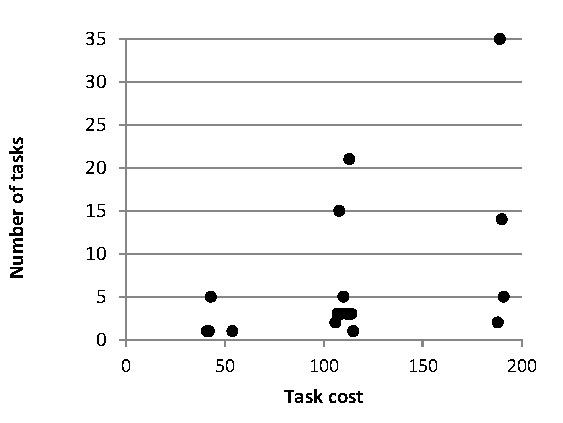
\includegraphics[width=\textwidth]{Figs/cholesky_8x8_distribution.pdf}
  \caption{Cholesky 8$\times$8}
  \label{cholesky8x8_dist}
\end{subfigure}
\begin{subfigure}[b]{0.3\textwidth}
  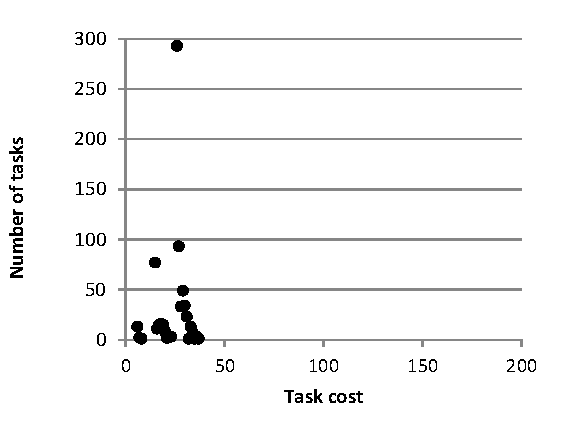
\includegraphics[width=\textwidth]{Figs/cholesky_16x16_distribution.pdf}
  \caption{Cholesky 16$\times$16}
  \label{cholesky16x16_dist}
\end{subfigure}
\begin{subfigure}[b]{0.3\textwidth}
  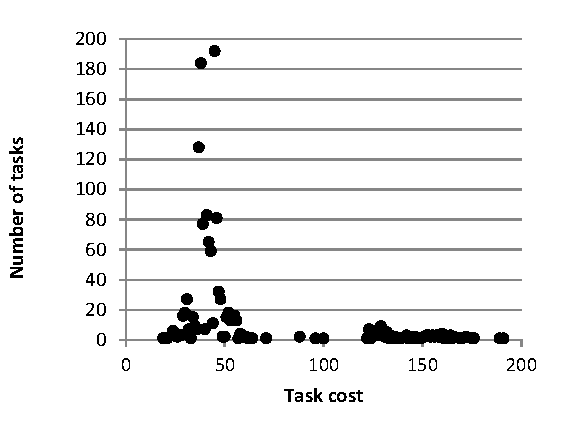
\includegraphics[width=\textwidth]{Figs/QR_16x16_distribution.pdf}
  \caption{QR factorization}
  \label{qr_dist}
\end{subfigure}
\begin{subfigure}[b]{0.3\textwidth}
  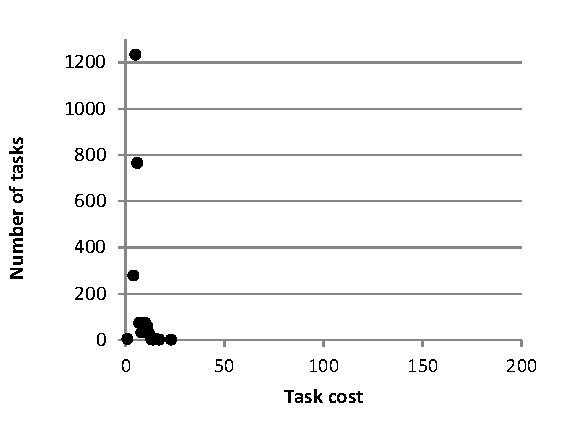
\includegraphics[width=\textwidth]{Figs/heat_16x16_distribution.pdf}
  \caption{Heat diffusion}
  \label{heat_dist}
\end{subfigure}
\begin{subfigure}[b]{0.3\textwidth}
  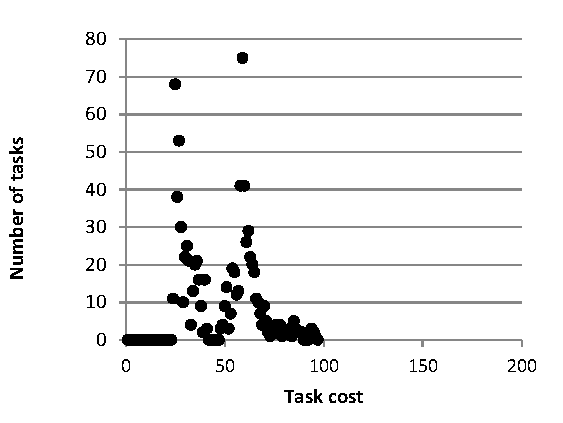
\includegraphics[width=\textwidth]{Figs/histogram_8x8_distribution.pdf}
  \caption{Integral Histogram}
  \label{histogram_dist}
\end{subfigure}
\begin{subfigure}[b]{0.3\textwidth}
  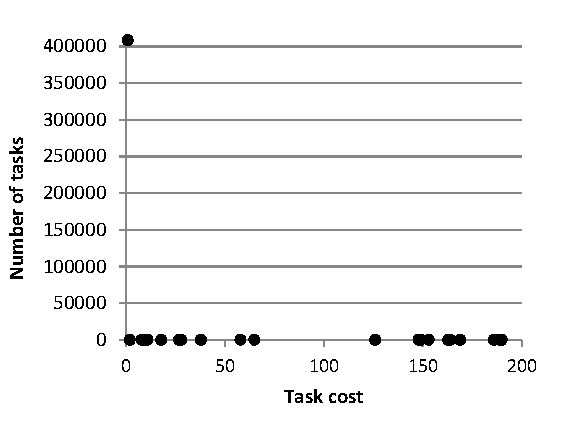
\includegraphics[width=\textwidth]{Figs/bodytrack_native_distribution.pdf}
  \caption{Bodytrack}
  \label{bodytrack_dist}
\end{subfigure}
  \caption{Task cost distribution for each application. Results are based on 4BIG-core executions. $x$ axis shows the cost of the tasks and $y$ axis shows the number of tasks with the corresponding task cost.}
  \label{distributions}
  \vspace{-0.4cm}
\end{figure*}


\begin{figure*}[!t]
  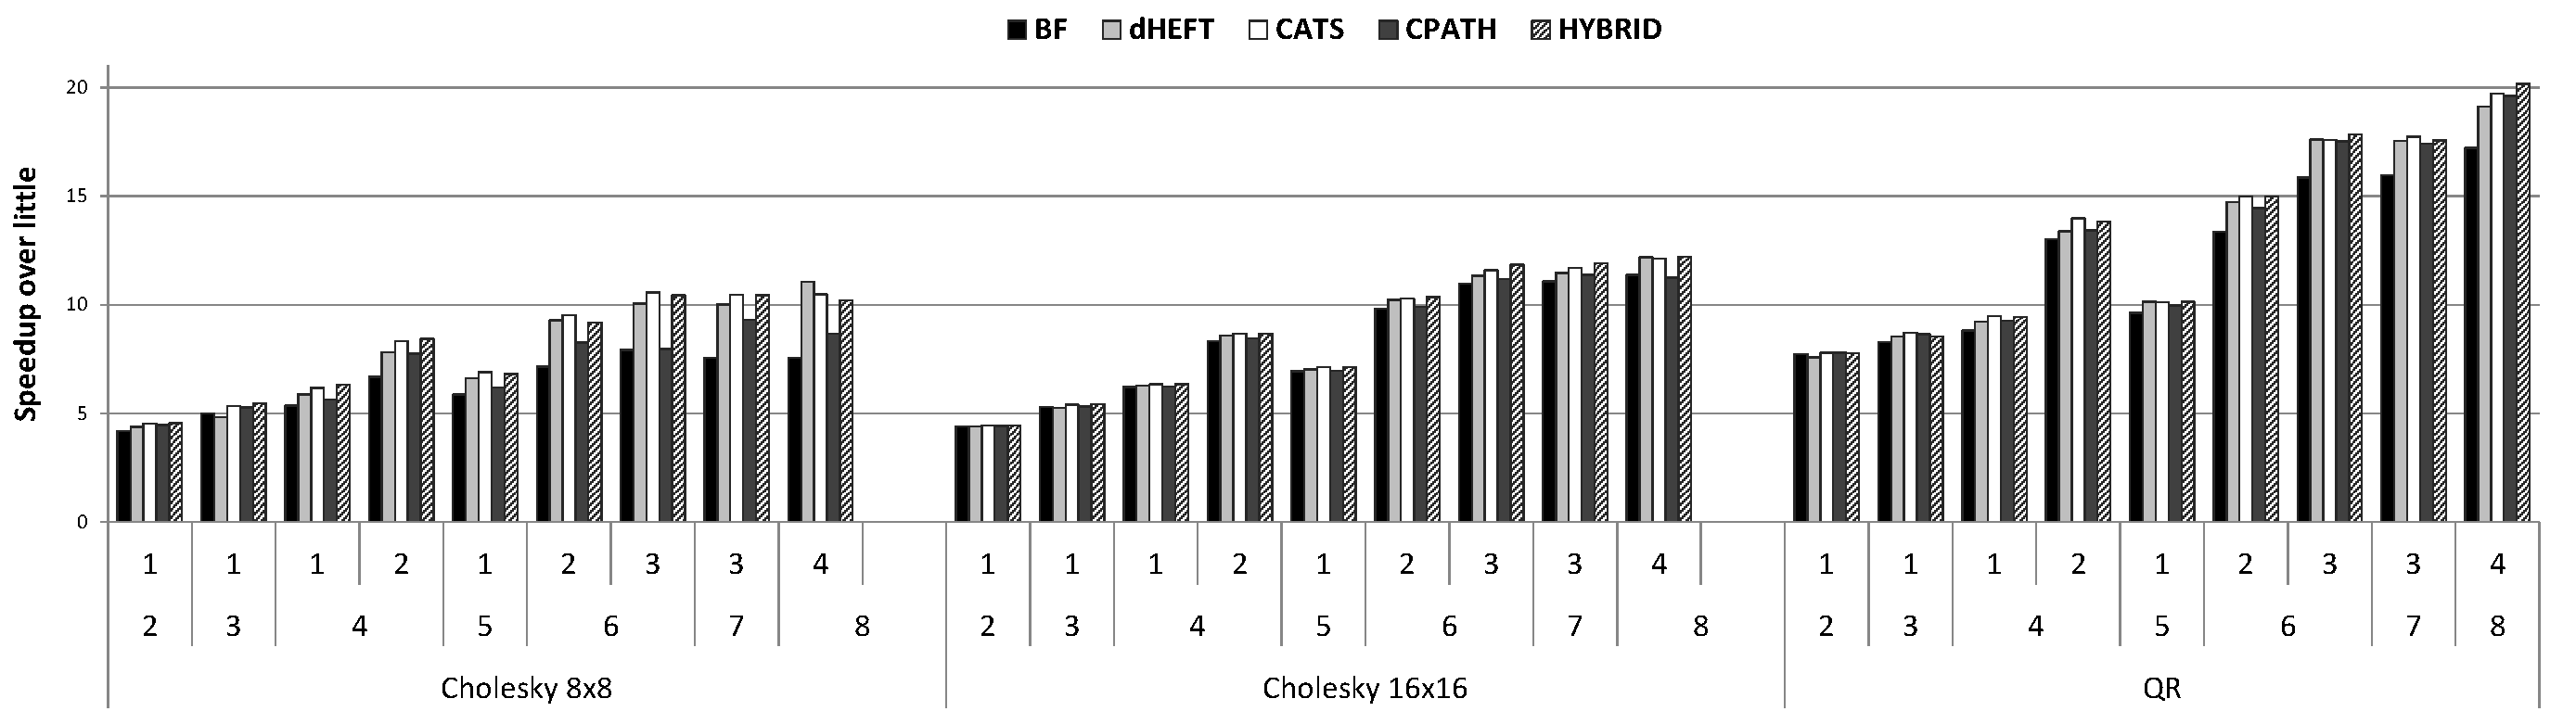
\includegraphics[width=\textwidth]{Figs/speedup_apps1.pdf}
   \vspace{-0.4cm}

  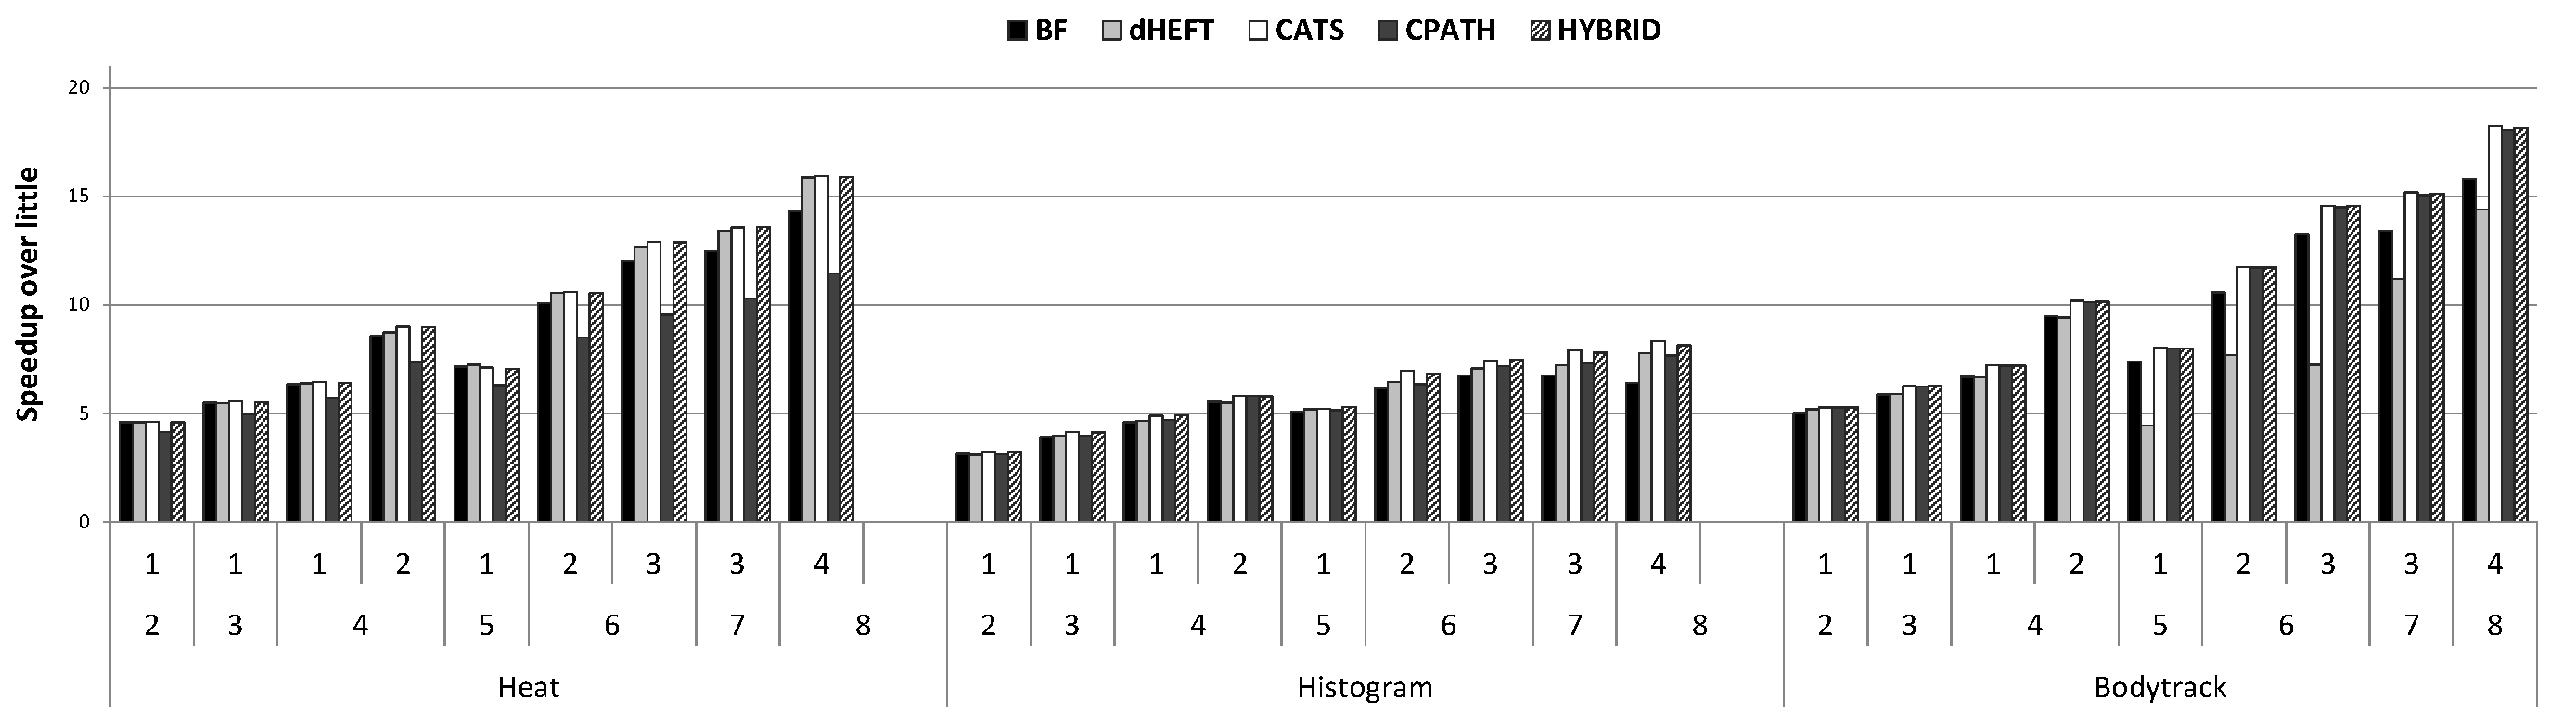
\includegraphics[width=\textwidth]{Figs/speedup_apps2.pdf}
  \caption{Speedups obtained for each scheduler and each application}
  \label{speedup}
  \vspace{-0.4cm}
\end{figure*}  

\subsubsection{Evaluation of Runtime Activity Manager}
In our preliminary evaluation of three workloads using RAM we observe very promising results.
Specifically, Figure~\ref{speedupRAM} shows the speedup of the baseline and RAM approach when we simulate the applications on up to 512 cores.
We can see that for the baseline runtime, performance saturates as we increase the number of cores. 
This happens due to the task creation overhead, which we overcome by accelerating it on the special hardware. 

\begin{figure*}[!t]
  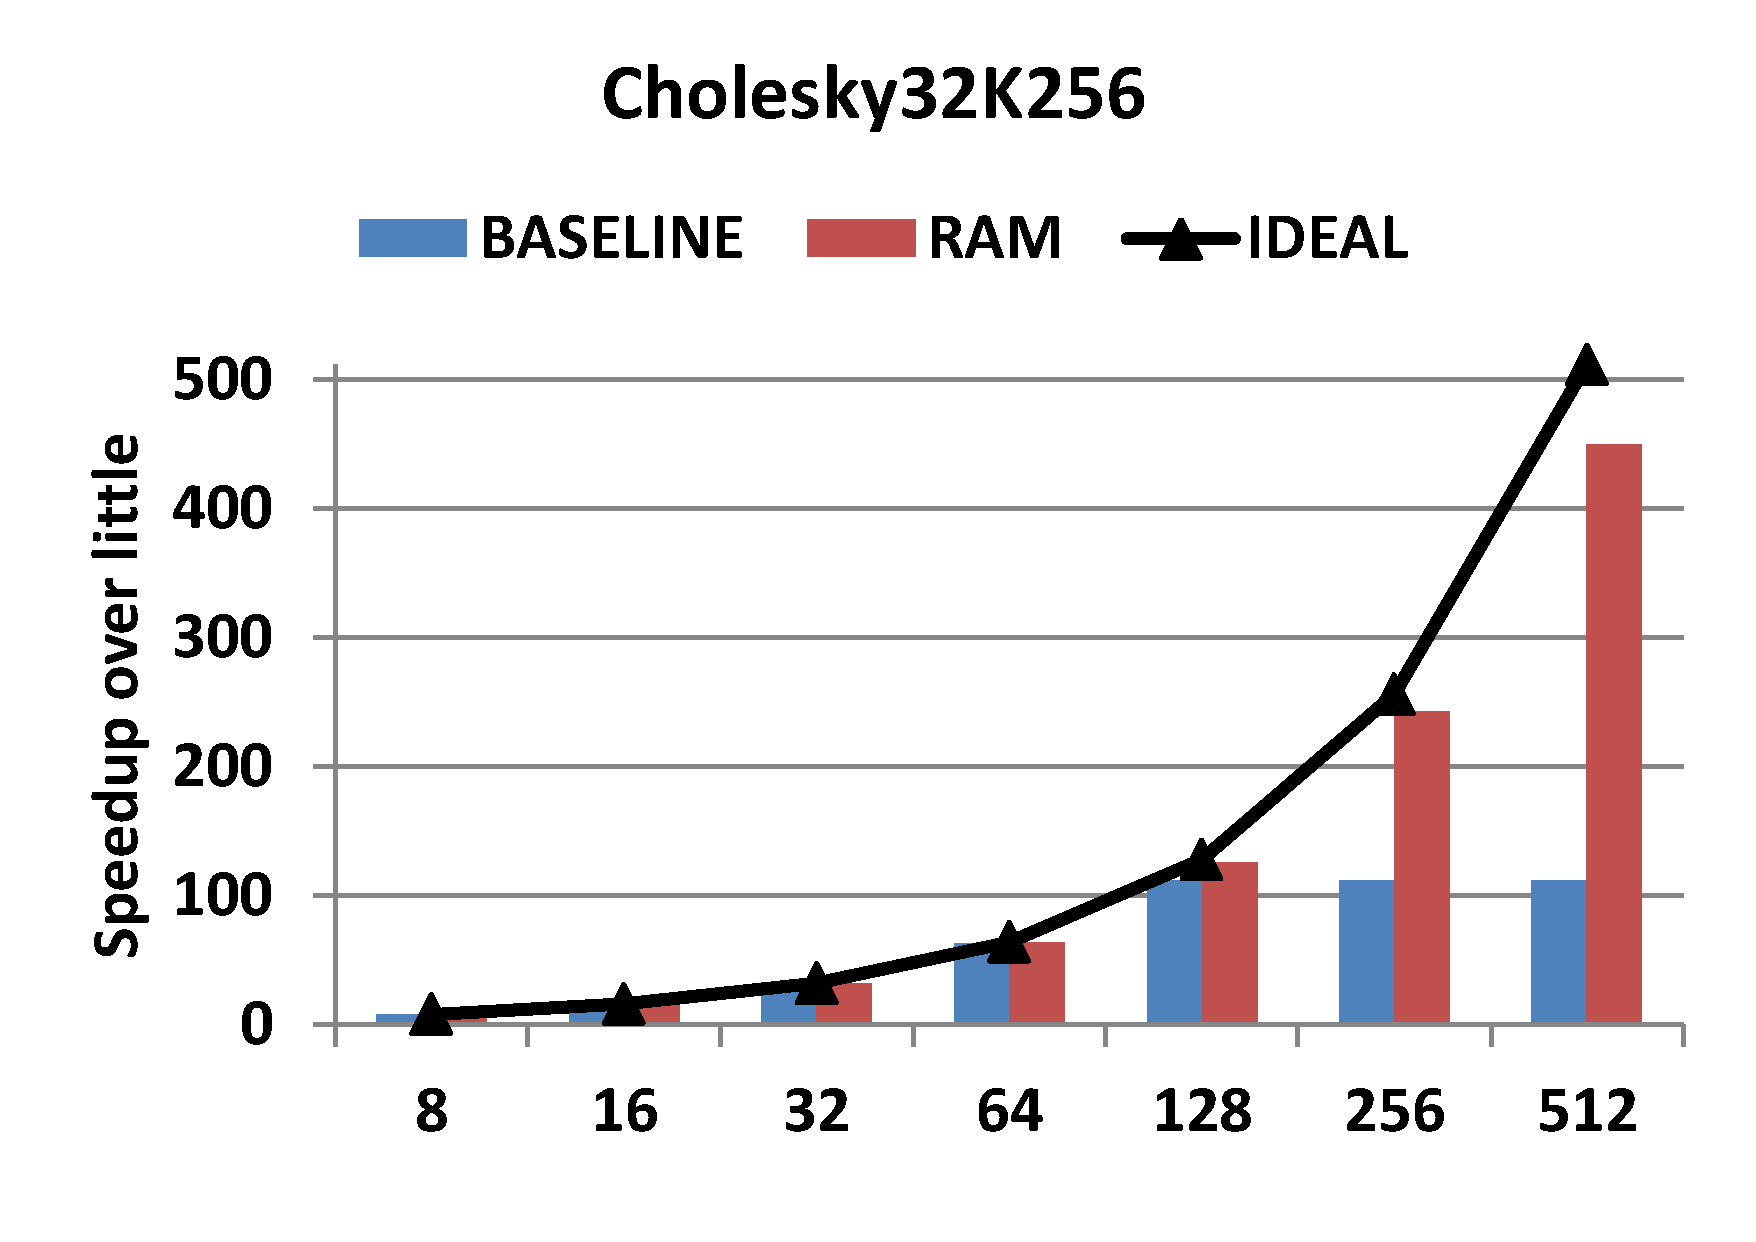
\includegraphics[width=0.32\textwidth]{Figs/cholesky_32K256.pdf}
  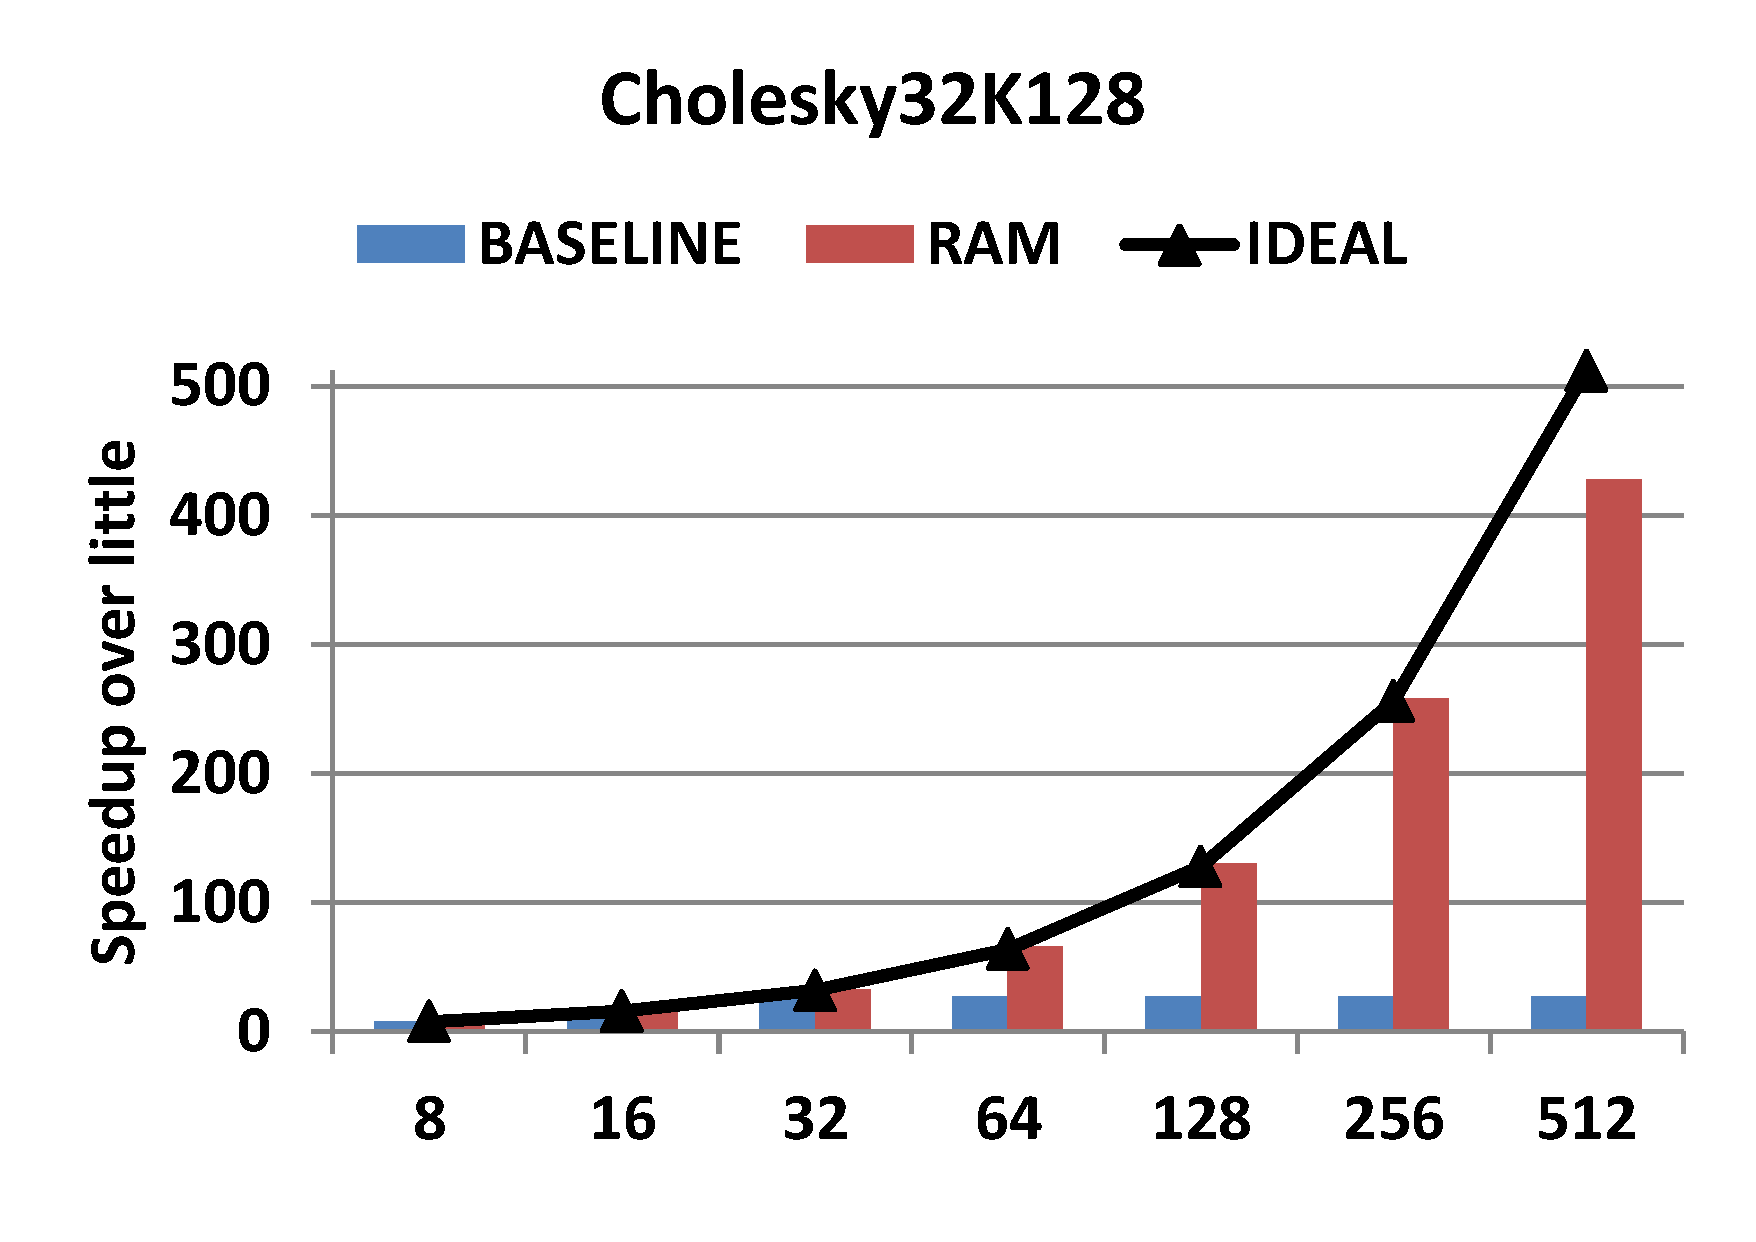
\includegraphics[width=0.32\textwidth]{Figs/cholesky_32K128.pdf}
  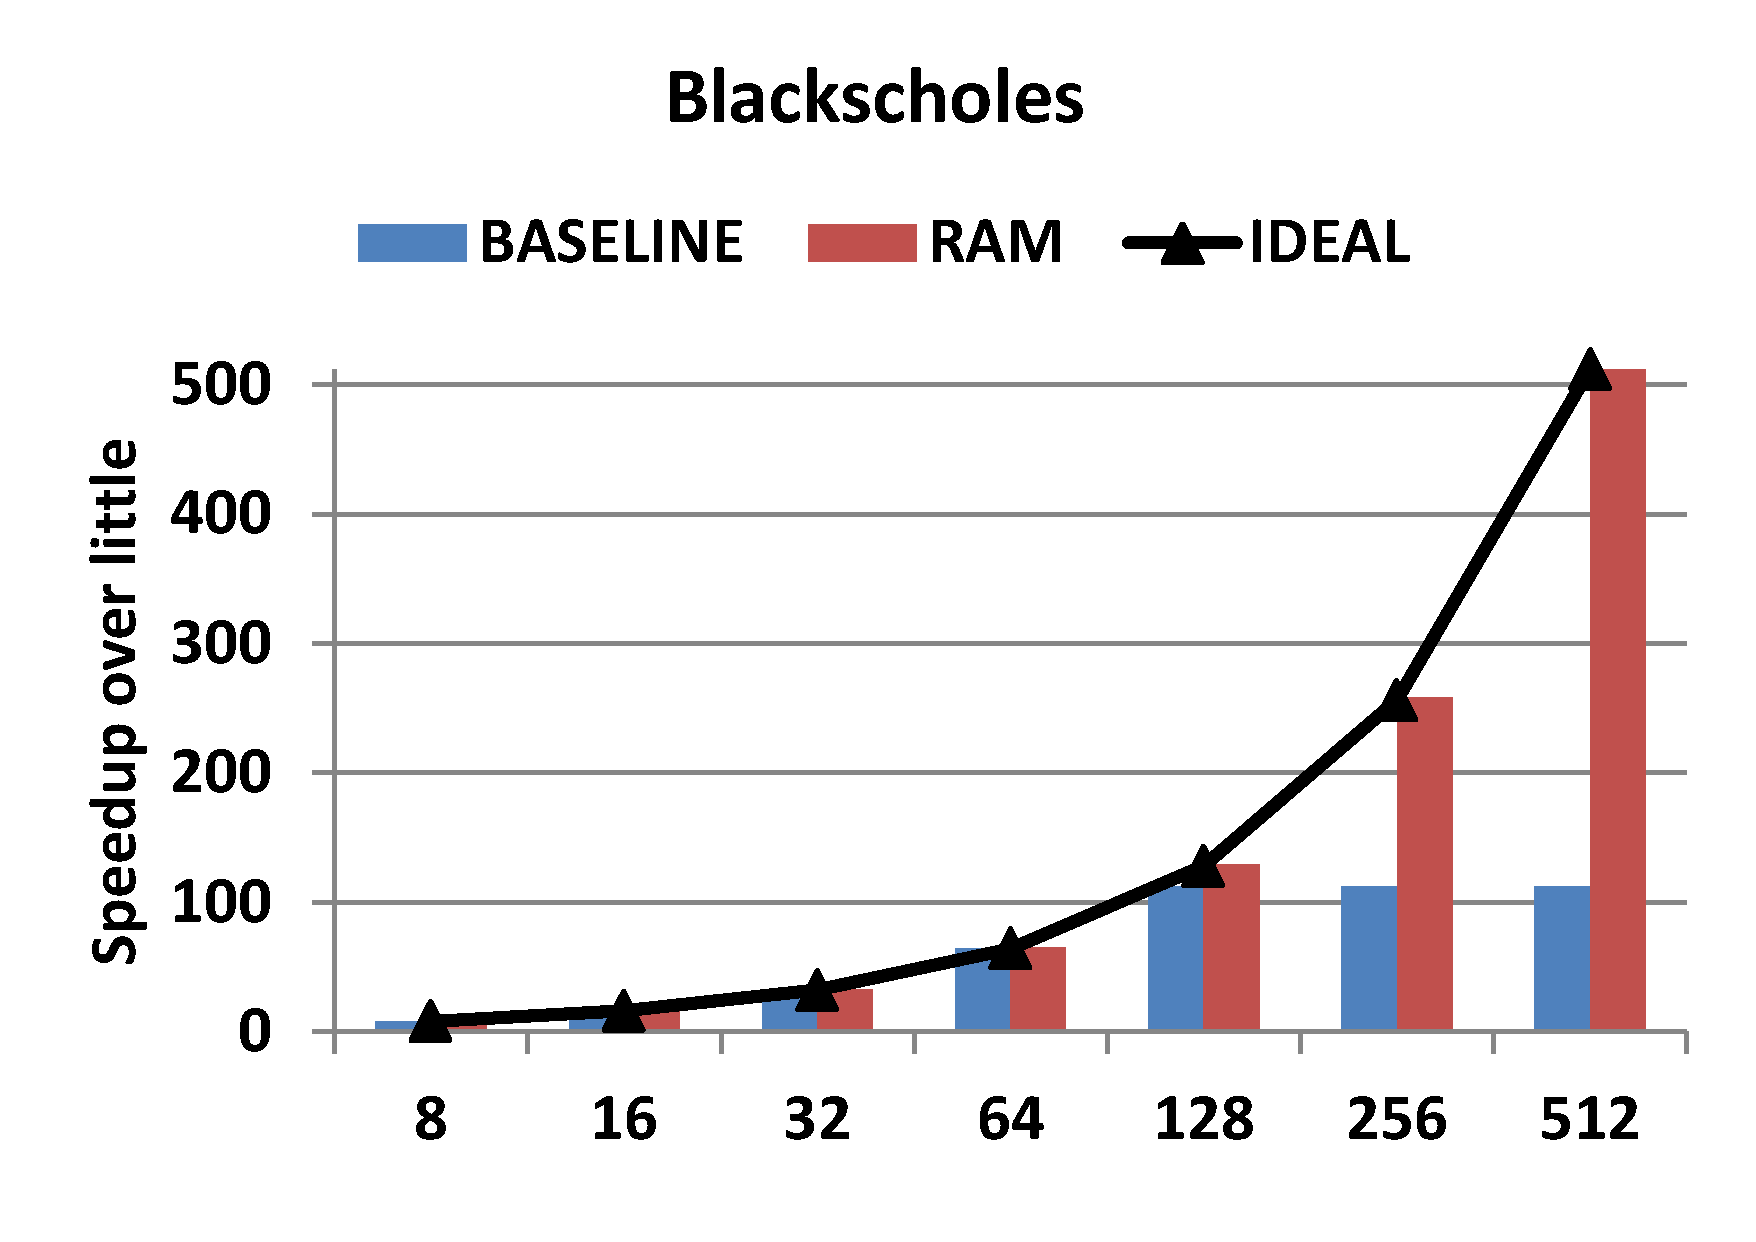
\includegraphics[width=0.32\textwidth]{Figs/blackscholes.pdf}
  \caption{Speedups obtained for default OmpSs runtime (BASELINE) and RAM for each application}
  \label{speedupRAM}
\end{figure*}  

We plan to further improve this evaluation by adding results for asymmetric systems.

\part{Epilogue}
\chapter{Conclusions}
This PhD thesis incorporated flexible software techniques on the runtime system level in order to effectively utilize asymmetric systems.
The main contributions of the thesis rely on the efficient exploitation of future asymmetric multi-core systems in terms of performance as well as on conceiving future asymmetric architectures that fit the needs of high performance computing.
\kc{TODO, ellaborate on:}
	%Our current results have shown that the state-of-the-art asymmetric multi-core systems are not ready to efficiently run out-of-the-box high performance applications and that the most efficient way is by using a task-based approach.
	%This increases the need of research in this direction through the paths of scheduling and thread migration as described in the previous Chapters.
	%In our first attempts to follow these paths, we have seen the high potential of the criticality-aware task schedulers to speed up dependency-intensive applications and take advantage of the asymmetric compute resources.

	This thesis showed that current highly parallel applications are not ready to fully utilize an AMC sytem. 
	Parallelizing on application level requires significant programming effort and results are not always optimal.
	Using task-based programming models offers a flexible solution for programmability as well as scheduling and performance. 
	Using task-based programming models on AMC systems increases the need of research for enhancing the runtime system of the task-based programming models to achieve even higher performance. 
	Scheduling and runtime overheads' acceleration are useful research lines towards this direction.
	
	Following these research lines, in this thesis we introduced three novel schedulers for asymmetric systems. 
	We implemented these schedulers within the OmpSs task-based programming model and used them on a real asymmetric multi-core system.
	These scheduling approaches do not consist of theoretical results but are implementable and work on real platforms with real applications, contrary to previous approaches that use synthetic TDGs and profiling. 
	CATS offers a consistent performance improvement of around 10\% to 20\% reaching up to 30\%.
	By tracking task execution time, CPATH offers a higher accuracy in the identification of critical tasks but this does not imply that it always increases performance. 
	The number of tasks, task cost variability as well as the TDG structure are vital characteristics of an application that affect performance, especially on AMC systems.

	Furthermore, an important outcome of this thesis is the proof that task creation is a significant bottleneck in parallel runtime systems.
	To overcome this significant bottleneck of task-based programming models we proposed TaskGenX, a HW-SW proposal for accelerating task creation that achieves up to 15$\times$ increased performance.
	TaskGenX is excels compared to existing approaches, for two main reasons; first is because it achieves higher performance as the number of cores is increased. 
	TaskGenX outperforms approaches that accelerate all the runtime activities by 54\% and approaches that accelerate scheduling and dependence analysis  by 70\%.
	The second reason that TaskGenX solution is optimal compared to other approaches is that it is the most minimalistic solution. 
	It achieves such results by only requiring the acceleration of task creation, using a simple single-core hardware proposal.
	Throughout TaskGenX study we also made observations that contribute and give guidelines for the design of the future multi-core asymmetric systems for high performance computing.

	Finally we showed that scheduling is important not only for asymmetric systems that run highly parallel applications, but it is also important and can increase performance when used on mobile devices for running multi-threaded applications such as games.
	An as simple scheduling approach as RTS of this thesis can achieve up to 7.5\% increase in FPS while maintaining stable temperature and high FPS stability.


%Existing parallel scientific applications will become portable when moving from a traditional multi-core to an asymmetric multi-core system. 
%Our useful observations throughout this study will also contribute and give guidelines for the design of the future multi-core asymmetric systems for high performance computing.

%goals are performance and energy efficiency as well as the portability of existing applications from the traditional homogeneous multi-cores to the new asymmetric multi-core systems.

%From our current results we have seen that current asymmetric multi-core systems are not ready to efficiently run out of the box high performance scientific applications and that the most efficient way is by using a task-based approach.
%Moreover, we have seen the potential of the criticality-aware task schedulers to speed up dependency-intensive applications and take advantage of the asymmetric compute resources is very high but sometimes comes at the cost of high additional overhead.
%We expect that adding one more scheduling layer will help eliminate the scheduling overheads of the smart heterogeneous scheduling approaches and boost performance and energy efficiency of such architectures.

%We are optimistic that following our second research approach of runtime thread migration will also contribute positively.
%The greatest challenge will be to increase performance without sacrificing energy, thus the dynamic search for the appropriate assistant core for the runtime thread has to consider all these obstacles.
%We expect that this approach will also influence designers to consider the use of assistant cores in the future asymmetric multi-cores.
%Finally, in our last and most complete approach we will need to synchronize all of our tools (e.g. scheduling and thread migration) to adapt to the runtime circumstances and boost performance with decent energy consumption.

%Since a part of this work is already complete, we expect that our goals will be successfully accomplished and this study will be a useful reference for the future research.



%Our approach on dynamic runtime thread migration will further improve performance and energy efficiency and we expect that it will 



%The goal for this PhD thesis is to incorporate techniques from approximate computing to improve the performance in the scientific computing domain without incurring too much energy consumption overhead or drastically altering the current parallel programming paradigm. 
%~\\ \\
%It is a slight paradigm shifting from the traditional scientific computing ideology: to execute applications in a very-high-precision fashion. By loosing some of the precision 
%restrictions at some points of the execution one is able to open up more parallelism to boost the performance with the help of the runtime system yet maintaining the quality of the final
%results.
%~\\ \\
%As a novel approach, we can see the obstacle that lies beyond. Identifying the degree of approximation, realizing the right type of approximation, the applicability of the techniques 
%etc. all are still big questions. Yet with a right mindset and the progress we already have we are confident towards this approach.



\section{Future Directions}

TaskGenX+CATS
%\include{Chapter5/chapter5}
%\include{Chapter6/chapter6}
%\include{Chapter7/chapter7}



% ********************************** Back Matter *******************************
% Backmatter should be commented out, if you are using appendices after References
%\backmatter

% ********************************** Bibliography ******************************
\begin{spacing}{0.9}

% To use the conventional natbib style referencing
% Bibliography style previews: http://nodonn.tipido.net/bibstyle.php
% Reference styles: http://sites.stat.psu.edu/~surajit/present/bib.htm

\bibliographystyle{apalike}
%\bibliographystyle{plainnat} % use this to have URLs listed in References
\cleardoublepage
\bibliography{References/references} % Path to your References.bib file


% If you would like to use BibLaTeX for your references, pass `custombib' as
% an option in the document class. The location of 'reference.bib' should be
% specified in the preamble.tex file in the custombib section.
% Comment out the lines related to natbib above and uncomment the following line.

%\printbibliography[heading=bibintoc, title={References}]


\end{spacing}

% ********************************** Appendices ********************************

%\begin{appendices} % Using appendices environment for more functunality
%\include{Appendix1/appendix1}
%\include{Appendix2/appendix2}
%\end{appendices}

% *************************************** Index ********************************
\printthesisindex % If index is present

\end{document}
